% Mit twoside als weitere Option werden die Seitenränder angepasst, sodass beidseitig gedruckt werden kann
\documentclass[pdftex,12pt,a4paper]{report}

% kann optional mit "german" als Sprache gewählt werden
\usepackage[]{dbstmpl}



\global\arbeit{Bachelor Thesis}
%\global\arbeit{Masterarbeit}
%\global\arbeit{Seminararbeit}




% Hier die eigenen Daten eintragen
\global\titel{Action-Head Learning on Frozen Vision-Language Models for an Autonomous Minecraft Agent}
\global\bearbeiter{Diego Cuenca}
\global\betreuer{Prof. Volker Tresp}
\global\aufgabensteller{AUFGABENSTELLERNAME}
\global\abgabetermin{30.06.2026}
\global\ort{Munich}
\global\fach{Computer Science}

\begin{document}

% Deckblatt
\deckblatt

% Erklaerung fuer das Pruefungsamt
% Bei Seminararbeiten nicht noetig
\erklaerung

% Zusammenfassung
\begin{abstract}
Vision-language models carry broad visual and semantic priors, which makes them
attractive backbones for embodied agents --- but turning one into an agent
usually means post-training the whole model on action data, tying it to a single
embodiment at substantial cost. This thesis asks how far the cheap alternative
goes: freeze the backbone, train only a small ($\sim$5M-parameter) action head by
behavioural cloning, and keep the whole study inexpensive enough to sweep on a
single rented GPU. Using Minecraft as a deliberately hard test bed, it runs a
$2\times2$ ablation over backbone (the joint LLaVA-1.5 versus the contrastive
CLIP) and language condition (task prompt versus none), evaluating every cell
both on held-out frames and in live MineRL rollouts.

Three findings emerge, each replicated across three training seeds. First, under
the minimal concatenating head that the controlled comparison holds fixed, the
contrastive backbone is the more effective controller --- CLIP collects dirt where
the matched LLaVA cell sits at the floor --- but this is a property of the head
read-out, not of the backbone: two alternative heads recover CLIP-comparable
collection from the same frozen LLaVA features, making the result a head-by-backbone
interaction rather than an intrinsic ranking. Second, language conditioning is
likewise a backbone effect --- only CLIP's separate text encoder yields a prompt
signal the head can act on (a $42$-point attack-rate shift, large in every seed),
while LLaVA stays flat across prompts even though the prompt is almost perfectly
decodable from its features. Third, and most robustly, these differences are
invisible offline: the four cells are a near-tie on frame metrics yet diverge from
a dug stack of dirt to nothing per episode in rollout --- a direct demonstration
that closed-loop evaluation measures what frame-level metrics miss. The study
characterises the cheap-and-frozen corner of the design space and does not claim
either backbone's ceiling under fine-tuning.
\end{abstract}

% Inhaltsverzeichnis (abhaengig von der Laenge des Dokuments)
\tableofcontents

% Hier beginnt der Hauptteil

% ======================================================================
% Chapter 1 -- Introduction
% Target: ~1 page (single section, no subsections).
% PST "classic drama" arc: setting -> problem -> why existing means fall
% short -> approach -> how it solves it (+ contributions) -> outline.
% Present tense, active voice, "we"/"one" (not "I"). VLM not LLM,
% "frozen" not "fine-tuning".
% ======================================================================

\chapter{Introduction}
\label{chap:intro}

Vision-language models acquire broad visual and semantic priors from
large-scale pretraining, yet they are optimised to produce text rather
than to act. Converting that perceptual competence into the ability to
pursue goals inside an interactive environment remains an open problem.

A common route turns a vision-language model into an agent by
post-training the entire backbone on action data, as JARVIS-VLA does for
Minecraft \cite{li2025jarvisvla}. This ties the model's knowledge to a
single embodiment and demands substantial compute. Full fine-tuning is
also risky in itself: updating a strong pretrained backbone can distort
the very features it depends on and weaken out-of-distribution behaviour
\cite{kumar2022finetuningdistortpretrainedfeatures}. Established Minecraft
agents show the two prevailing alternatives, either training a large
control policy from scratch on human video \cite{baker2022vpt} or
bypassing pixel control through symbolic scripting interfaces. Neither
isolates how much agent competence already resides in a frozen,
general-purpose backbone.

This thesis introduces R1V-A, an agent that keeps the vision-language
backbone entirely frozen and trains only a small action head, on the
order of five million parameters, by behavioural cloning on recorded
Minecraft gameplay (rendered by a STEVE-1/VPT agent, not a human; see
Chapter~\ref{chap:method}). Each decision is conditioned on a single rendered
frame together with a natural-language task prompt, and no reward signal
is used during training.

Because the backbone never changes, its features can be computed once and
reused, which makes training cheap enough to sweep several configurations.
The frozen design also turns the backbone into a controlled variable,
which we exploit to make three contributions. First, we compare a joint
vision-language backbone (LLaVA-1.5) against a contrastive one (CLIP) used
purely as frozen feature extractors. Second, we ablate the language
pathway by training each backbone with and without the task prompt, asking
whether the prompt adds signal over image-only control. Third, we evaluate
the resulting agents not only on held-out frames but in live MineRL
rollouts, which probe the out-of-distribution behaviour that frame-level
metrics overlook.

Concretely, the thesis poses three research questions, one per contribution:
\begin{itemize}
\item \textbf{RQ1 (backbone).} Used only as a frozen feature extractor for a
small behavioural-cloning head, does a joint vision-language backbone
(LLaVA-1.5) yield a more capable Minecraft agent than a contrastive one (CLIP)?
\item \textbf{RQ2 (language).} Does conditioning the head on a natural-language
task prompt measurably change the agent's behaviour, and does the answer depend
on the backbone?
\item \textbf{RQ3 (evaluation).} Do live in-environment rollouts reveal
differences between these agents that held-out frame-level metrics do not?
\end{itemize}

The remainder of this thesis is organised as follows.
Chapter~\ref{chap:background} reviews the imitation-learning setting the
agent operates in, Minecraft as a control benchmark, the frozen
vision-language backbone and the rationale for freezing it, the
vision-language-action lineage the design descends from, and the factored
action space it predicts over. Chapter~\ref{chap:method} details the
problem formulation, the frozen-backbone architecture and trainable action
head, the training objective, the data pipeline, and the
rollout-evaluation protocol. Chapter~\ref{chap:experiments} reports the
$2\times2$ backbone-by-language ablation across both tasks, with
frame-level metrics and in-environment rollout results.
Chapter~\ref{chap:discussion} interprets these results, in particular what
they imply about the contribution of the language pathway and the choice
of frozen backbone. Chapter~\ref{chap:conclusion} summarises the findings
and outlines directions for future work.

% ======================================================================
% Chapter 2 -- Background
% Target: ~5 pages, <=25% of total. British spelling, present tense,
% active voice, "we"/"one". Every heading opens with a lead-in.
% [VERIFY] = key not yet confirmed in .bib.
% ======================================================================

\chapter{Background}
\label{chap:background}

% TODO: opening motivation paragraph (vision-LANGUAGE model not LLM;
%       "state cues"; BC is the algorithm) + chapter lead-in naming the
%       five threads. (Thesis-wide outline goes in the Introduction.)


% ----------------------------------------------------------------------
\section{Imitation Learning and Behavioural Cloning}
\label{sec:bg-il}
In the absence of a reward signal, an agent can still induce a policy from
expert demonstrations through a supervised learning algorithm, a setting
known as behavioural cloning \cite{Bain1995AFF}. The policy is trained to
reproduce the expert's action at each observed state. A well-documented
weakness of this approach is a compounding-error phenomenon: once the agent
commits an early mistake at deployment, it reaches states the expert
demonstrations never covered, where its predictions degrade further and
errors accumulate over the episode \cite{ross2011}. Formally, if the learned
policy incurs an error probability $\varepsilon$ on states drawn from the
expert distribution, the expected cost of behavioural cloning grows as
$\mathcal{O}(\varepsilon T^2)$ over a horizon of $T$ steps, since each
mistake compounds the mismatch between the states the agent visits and those
the expert demonstrated \cite{ross2011}. This offline-to-online gap is
observed empirically in Minecraft behavioural cloning \cite{kanervisto2020},
and it motivates evaluating the policy through in-environment rollouts
(Section~\ref{sec:rollout}) rather than held-out-frame metrics alone.

This vulnerability is sharper still when the policy conditions on a single
observation: with no temporal context, the agent cannot tell where in a
motion it is, so a momentary perceptual ambiguity can divert it into the
out-of-distribution regime described above. R1V-A operates in exactly this
single-frame regime, which motivates the past-action conditioning and
action-chunking mechanisms introduced in Chapter~\ref{chap:method}.

More recent analysis qualifies how fundamental this gap is. The quadratic
error growth is not intrinsic to behavioural cloning but depends on the
training loss: under a logarithmic loss the dependence on the horizon can be
substantially milder \cite{foster2024horizon}, although this guarantee
weakens again for the continuous action components that policies such as
R1V-A must predict \cite{simchowitz2025pitfalls}. The compounding-error view
therefore remains the appropriate framing here.


% ----------------------------------------------------------------------
\section{Minecraft as a Learning Environment}
\label{sec:bg-minecraft}
Minecraft has emerged as a demanding control benchmark for embodied agents,
owing to its open-ended environment, partial observability, long task
horizons, and large diversity of objectives \cite{fan2022minedojo}. Early
agents achieved competent play through symbolic or scripted interfaces that
abstract away perception and low-level control. A more recent line instead
requires the agent to act from raw pixels through the same
keyboard-and-mouse interface a human uses, a substantially harder setting
that VPT established at scale by behavioural cloning on large quantities of
human gameplay video \cite{baker2022vpt}. R1V-A belongs to this
pixel-and-keypress tradition.

Acting through this interface requires a policy to control the same inputs a
human does: a set of binary key presses together with continuous mouse
movement. VPT formalises this as a factored action space of discrete key
toggles plus a two-axis camera signal, and discretises each camera axis into
mu-law-spaced bins so that the long-tailed distribution of human mouse
movements is represented at higher resolution near zero \cite{baker2022vpt}.
R1V-A adopts this action space and bin convention directly
(Section~\ref{action_space}). Human demonstrations for this setting are
commonly logged in the BASALT contractor format, in which each frame is
paired with the action the player executed, with camera magnitudes already
snapped to the VPT bin centres \cite{shah2021basalt}. The recordings used in
this work follow this convention, so the action logs map onto the policy's
output representation without loss.
% TODO: lifshitz2023steve1 is uncited -- place it (language-for-task-spec
%       example) or drop it from the chapter.


% ----------------------------------------------------------------------
\section{Vision-Language Models and the Frozen-Backbone Paradigm}
\label{sec:bg-vlm}
R1V-A treats a pretrained vision-language model as a fixed feature extractor
and trains only a small head on its representations. This section introduces
the two families of vision-language model the experiments compare, which
differ in how they combine image and text, and then sets out why freezing
such a model is a sound choice.

\subsection{Contrastive and Joint Vision-Language Models}
\label{subsec:bg-vlm-families}
Since we wish to compare the contribution of language to an agent's
capabilities, we examine two structurally different ways of relating images
and text. The two backbones we ablate, CLIP and LLaVA, sit at opposite ends
of a fusion spectrum, and the distinction governs how, and whether, a task
prompt can influence the visual representation.

CLIP \cite{radford2021clip} couples two independent encoders. A text encoder
maps a caption to a single embedding, taken from the activations at the
end-of-sequence position, and a vision encoder (a ViT) maps an image to a
single embedding via its pooled representation. Both are projected into a
shared space. Training is contrastive: for a batch of $N$ image-text pairs,
one forms the $N \times N$ matrix of cosine similarities between every text
and every image embedding, then maximises the $N$ diagonal entries, the true
pairs, against the off-diagonal mismatches. The two modalities therefore
never interact within an example; alignment emerges only through comparison
across the batch, and fusion amounts to a single dot product in the shared
space. A consequence we rely on later is that CLIP's image embedding is a
fixed, language-aligned summary of the frame, computed without reference to
any prompt.

LLaVA \cite{liu2023llava} instead injects vision into a language model. It
reuses a CLIP vision encoder to produce a sequence of patch features,
projects them into the word-embedding space of the language model, and
concatenates these visual tokens with the embedded prompt tokens. The
combined sequence passes through the language model, whose self-attention
layers process the image and text tokens as one sequence, so the two
modalities are jointly contextualised at every layer rather than only at the
output. Fusion here is deep rather than late. The follow-up LLaVA-1.5
\cite{liu2024improvedbaselinesvisualinstruction} keeps this design and
strengthens it, replacing the original single linear projection with a
two-layer multilayer perceptron and broadening the instruction-tuning data
with academic visual-question-answering tasks; this is the backbone R1V-A
uses. This difference in fusion motivates our ablation. In CLIP the prompt
enters only as a parallel embedding, whereas in LLaVA it shares a sequence
with the image inside the model, so the question of whether the prompt
carries usable signal is distinct for the two backbones.

\subsection{Freezing Strong Pretrained Features}
\label{subsec:bg-freeze}
Adapting a large pretrained model to a new task need not mean updating its
weights. Full fine-tuning, the standard approach, carries a documented risk:
when the pretraining and downstream distributions differ, updating all
parameters can distort the pretrained features and degrade performance on
inputs that fall outside the fine-tuning data, the very generalisation a
large backbone is meant to provide
\cite{kumar2022finetuningdistortpretrainedfeatures}. Since R1V-A is evaluated
in rollout worlds it never saw during training, preserving that
out-of-distribution generalisation is a direct concern.

Freezing the backbone and training only a lightweight module on top avoids
this risk and has an established precedent in vision-language modelling.
BLIP-2 connects a frozen image encoder to a frozen language model through a
small trainable bridge, reaching competitive performance while leaving both
large components untouched
\cite{li2023blip2bootstrappinglanguageimagepretraining}. The same principle
underlies R1V-A: the vision-language backbone is held fixed and only the
action head receives gradients.

Freezing is the strict end of a spectrum of parameter-efficient adaptation.
Methods such as LoRA occupy the middle, injecting a small number of trainable
low-rank updates into an otherwise frozen backbone, which adapts the model at
a fraction of the cost of full fine-tuning \cite{hu2022lora}. R1V-A takes the
most conservative position on this spectrum, leaving every backbone parameter
unchanged, which both eliminates the distortion risk entirely and makes the
cached-feature training scheme of Chapter~\ref{chap:method} possible.


% ----------------------------------------------------------------------
\section{Vision-Language-Action Models}
\label{sec:bg-vla}
The frozen backbone and trainable action head together form a
vision-language-action (VLA) model: a system that maps visual and
linguistic input to control output. R1V-A descends from a recent line of
such models, and this section places it within that lineage and against its
closest Minecraft relatives.

The VLA pattern emerged first in robotics, where a vision-language backbone
is repurposed to emit actions rather than text. RT-2 established the
template by training a large vision-language model to output robot commands
as if they were language tokens, transferring web-scale visual and semantic
knowledge into control \cite{brohan2023rt2}. OpenVLA showed the approach
scales as an open recipe at the seven-billion-parameter range comparable to
R1V-A's backbone, adapting the model with low-rank updates rather than full
retraining \cite{kim2024openvla}. Closer to R1V-A's design, RoboFlamingo
keeps the vision-language backbone largely fixed and trains a separate
policy head on top \cite{li2023roboflamingo}, and LLaRA builds a VLA
directly on a LLaVA-style backbone \cite{li2024llara}, while $\pi_0$
attaches a lightweight action module to a frozen model \cite{black2024pi0}.
R1V-A shares this frozen-backbone, separate-head philosophy, but applies it
to Minecraft rather than physical manipulation.

Within Minecraft, two systems frame the design space this thesis works in. PR2L
is the closest published precedent and the methodological template for this
work: it pairs a frozen vision-language model with a learned policy to act from
pixels \cite{chen2024pr2l}, and as in PR2L the contribution here is comparative
and diagnostic --- which frozen backbone yields a usable signal, and how that
signal behaves in closed-loop rollouts --- rather than a new architecture.
JARVIS-VLA sits at the opposite end of the same axis: it fully post-trains the
vision-language backbone on Minecraft data \cite{li2025jarvisvla}, whereas R1V-A
leaves the backbone entirely frozen. It is a conceptual contrast rather than a
benchmarked baseline --- this thesis reproduces no JARVIS-VLA result and does not
measure the full post-training-versus-frozen trade-off that a true head-to-head
would require, confining its conclusions to the frozen regime it actually
studies.

\subsection{Does the Language Pathway Help?}
\label{subsec:bg-language}
A VLA receives a language prompt alongside its visual input, but it does not
follow that the prompt changes what the agent does. Prior work on
language-conditioned imitation finds that a natural-language goal can improve
a policy when tasks must be distinguished, yet image-only policies often
remain strong baselines, since much of the task is already legible from the
visual state alone \cite{lynch2021langlfp}. For R1V-A the question is
sharpened by the frozen-backbone setting: the prompt can only help if the
fixed backbone already encodes it in a form the action head can read.
Whether it does so is what the prompt ablation in Chapter~\ref{chap:method}
measures.

\subsection{Action Chunking}
\label{subsec:bg-chunking}
The compounding-error problem of Section~\ref{sec:bg-il} grows with the
number of independent decisions an agent makes over an episode. Action
chunking attacks this directly: instead of predicting one action per step,
the policy predicts a short sequence of future actions in a single forward
pass, executes the first, and re-plans on the next observation. Introduced by
ACT for fine-grained imitation, this shortens the effective decision horizon
and lets the policy commit to locally coherent motions rather than
re-deciding from scratch at every frame \cite{zhao2023act}. R1V-A adopts the
predict-a-chunk, execute-the-first recipe, which is a particularly natural
fit for its single-frame setting, where consecutive observations carry
little new information and short bursts of action are highly predictable.


% ----------------------------------------------------------------------
\section{Factored Action Spaces and Multi-Label Prediction}
\label{sec:bg-action}
A policy that controls a keyboard faces a combinatorial output space: with
$k$ keys, the set of possible key combinations is $2^k$, far too large to
treat as a single categorical choice. The standard remedy is to factor the
action space, predicting each component independently rather than enumerating
their joint configurations.

Action branching applies this idea by giving each discrete action dimension
its own output head, so the number of predictions grows linearly in the
number of keys rather than exponentially \cite{tavakoli2018actionbranching}.
R1V-A predicts each key as an independent binary decision, which also matches
the structure of the data: a human routinely holds several keys at once, for
example moving forward while attacking, so the targets are genuinely
multi-label rather than mutually exclusive. The head is therefore trained
with a binary cross-entropy loss applied per key, the natural objective for
independent binary outputs.

The two continuous camera axes are handled separately. Following the VPT
convention, each axis is discretised into mu-law-spaced bins and predicted as
a categorical distribution, so that camera control becomes a classification
problem alongside the keys rather than a regression
\cite{baker2022vpt}. This keeps the entire action head within a single
classification framework and lets the mu-law spacing devote finer resolution
to the small movements that dominate human play.


% ----------------------------------------------------------------------
% OPEN ITEMS (still to do):
%  - Write the chapter opening paragraph + chapter lead-in (top of file).
%  - Place or drop lifshitz2023steve1 (2.2).
%  - Add zhao2023act to .bib.
%  - Resolve all [VERIFY] keys against the .bib.
%  - MineDreamer provenance -> Method Dataset section (not here).
%  - Check VLA acronym is not also expanded in the Introduction.
%  - OPTIONAL: justify plain BCE vs reweighted losses (focal/asymmetric)
%    in 2.5 only if you want to cite ridnik2021asymmetric / lin2017focal.
% ----------------------------------------------------------------------
\chapter{Method}
\label{chap:method}
\section{Problem Formulation}

I frame the task as imitation learning from recorded gameplay demonstrations
\cite{Bain1995AFF}. At each timestep $t$, the agent observes an RGB frame
$s_t$ of resolution $360 \times 640 \times 3$, paired with a natural-language
task prompt $p$ describing the goal (e.g.\ \enquote{collect dirt}). The agent
must predict an action $a_t \in \{0,1\}^{21} \times \mathbb{R}^2$, comprising
21 binary key presses and 2 continuous camera magnitudes $(c_x, c_y)$. The
training signal is a dataset of demonstrations
\begin{equation}
    \mathcal{D} = \{(s_t,\, p,\, a_t)\}_{t=1}^{N},
\end{equation}
where each frame is paired with the action the demonstrator executed at that
timestep. No reward signal is available; the learner can only infer
$\hat{\pi}$ from the state-action pairs in $\mathcal{D}$. I therefore adopt
Behavioural Cloning (BC) as my learning algorithm.

The policy does not consume visual history: only the current frame $s_t$ is
encoded by the backbone. To partially compensate, the head is conditioned on
a short window of past actions and predicts a short chunk of future actions,
as described in Sections~\ref{past_action} and~\ref{chunking}.

Finally, I note that the absence of expert querying during training can lead
to \textit{compounding errors}: once the agent deviates from states seen in
$\mathcal{D}$, it finds itself in an out-of-distribution region from which it
cannot recover \cite{ross2011}. This offline-to-online gap is a fundamental
property of plain BC, where errors scale as $\mathcal{O}(\varepsilon T^2)$
with horizon $T$, and motivates both the action-chunking design choice in
Section~\ref{chunking} and the in-environment rollout evaluation in
Section~\ref{sec:rollout}.

\section{Architecture} \label{sec:architecture}

\subsection{Frozen Vision-Language Backbone} \label{sec:backbone}
Freezing strong pretrained representations and training only a lightweight
head has been shown to match or exceed full fine-tuning accuracy while
remaining computationally
tractable~\cite{kumar2022finetuningdistortpretrainedfeatures}, a paradigm
established in vision-language modelling by
BLIP-2~\cite{li2023blip2bootstrappinglanguageimagepretraining}. I adopt
LLaVA-1.5-7B~\cite{liu2024improvedbaselinesvisualinstruction}, which pairs a
CLIP-ViT-L-336px vision encoder with a Vicuna-7B language decoder, as the
primary frozen backbone. Each state $(s_t, p)$ is passed jointly through
\texttt{LlavaProcessor} and the autoregressive decoder, where the single
\texttt{<image>} placeholder is expanded to 576 visual tokens that are
processed alongside the prompt tokens through all decoder layers. I read the
post-normalisation hidden states of the final layer via a forward hook on the
decoder's terminal RMSNorm.

Because the LLaMA decoder exposes no CLS token, a fixed-size summary must be
pooled from the token sequence. A naive mean over the full joint sequence is
dominated by the roughly 576 visual tokens and washes out the handful of
prompt tokens. I therefore pool the image-role and text-role tokens
\emph{separately} using their attention masks and concatenate the two
4096-dimensional means:
\begin{equation}
    \phi_{\mathrm{LLaVA}}(s_t, p) = \bigl[\, \overline{h}^{(L)}_{\mathcal{I}}\,;\;
    \overline{h}^{(L)}_{\mathcal{T}} \,\bigr] \in \mathbb{R}^{8192},
\end{equation}
where $\overline{h}^{(L)}_{\mathcal{I}}$ and $\overline{h}^{(L)}_{\mathcal{T}}$
are the masked means of the final-layer hidden states over the image-role
token set $\mathcal{I}$ and the text-role token set $\mathcal{T}$, each of
dimension 4096. Split-pooling keeps the language signal as an explicit,
undiluted component of the representation, mirroring the concatenated layout
of the contrastive baseline below. All 7B backbone parameters are frozen
throughout training, so only the action head defined in
Section~\ref{action_head} receives gradient updates.

\subsection{Contrastive Vision-Language Baseline} \label{sec:clip_baseline}
To isolate the contribution of LLaVA's joint vision-language reasoning from
its raw visual features, I include a frozen CLIP-ViT-L/14
baseline~\cite{radford2021clip} as a comparison backbone. Whereas LLaVA fuses
image and text inside a single autoregressive decoder, CLIP encodes the two
modalities with separate encoders that have only been aligned by contrastive
pretraining. The image encoder produces a 768-dimensional pooled image
embedding $\phi_v(s_t)$ and the text encoder produces a 768-dimensional
pooled text embedding $\phi_t(p)$. I concatenate the two to form the joint
representation
\begin{equation}
    \phi_{\mathrm{CLIP}}(s_t, p) = \bigl[\,\phi_v(s_t);\; \phi_t(p)\,\bigr] \in \mathbb{R}^{1536}.
\end{equation}
When the prompt is ablated (Section~\ref{ablation}), the text branch is
replaced with a zero vector of the same dimensionality rather than removed,
so the head input shape is held constant across language conditions and only
the backbone choice is varied. Because the CLIP image encoder is separate
from the text encoder, its visual features never attend to the prompt; this
is the key respect in which the no-prompt condition differs between the two
backbones (Section~\ref{ablation}).

\subsection{Action Space} \label{action_space}
The MineRL environment exposes a hybrid action space inherited from
VPT~\cite{baker2022vpt}: 21 binary keys (movement, attack, use, hotbar
selection, inventory toggle, ESC) and 2 continuous camera magnitudes
$(c_x, c_y) \in \mathbb{R}^2$ controlling view pitch and yaw. Predicting the
21 binary keys jointly as a single categorical distribution over all $2^{21}$
combinations is intractable; following the action-branching paradigm of
Tavakoli et al.~\cite{tavakoli2018actionbranching}, I instead predict each
key independently via its own sigmoid output, which scales linearly rather
than combinatorially in the number of keys.

The continuous camera axes are handled separately. Rather than regressing
$(c_x, c_y)$ directly, I discretise each axis into 11 mu-law-spaced bins
following the VPT convention~\cite{baker2022vpt}, allowing the policy to
represent the bimodal \enquote{stay still vs.\ turn} structure of human
demonstrations that a regression loss would collapse to the mean. Each axis
is therefore predicted as a categorical distribution over 11 bins, decoded
back to degrees at rollout time via the mu-law inverse. This yields the
per-step output dimensionality $D = 21 + 2 \times 11 = 43$.

\subsection{Past-Action Conditioning} \label{past_action}
A single frame is often insufficient to disambiguate the current action under
behavioural cloning. Tasks such as \texttt{collect\_dirt} and
\texttt{chop\_a\_tree} are dominated by long, repetitive action runs:
attack sequences of roughly 30 ticks while breaking a block, forward runs of
50 to 200 ticks while traversing the world, and small camera adjustments when
tracking a stationary target. Within such a run, consecutive frames are
visually near-identical, yet the correct action is overwhelmingly to repeat
the previous one. The conditional probability $\Pr(a_t = 1 \mid a_{t-1} = 1)$
is much higher than the marginal $\Pr(a_t = 1)$ for these sticky actions, but
single-frame BC only learns the marginal.

I therefore condition the action head on the last $K = 8$ executed actions.
Each past action is encoded as a $D = 43$ dimensional vector matching the
per-step output layout: the 21 binary keys as $0/1$ indicators (several of
which may be active at once) and each of the two camera axes as a one-hot
over its 11 mu-law bins. The resulting $K \times D$ matrix is flattened and
concatenated to the pooled backbone feature $\phi(s_t, p)$ before the head.
The window is zero-padded at trajectory start and right-aligned so the most
recent action occupies the last slot. This signal is intentionally injected
at the head input rather than appended to the text prompt. The head receives
the $K \cdot D = 344$ dimensional past-action vector as a dedicated
full-strength input to its trainable weights, whereas the same information
expressed as prompt text would have to be encoded and summarised by the
frozen backbone, competing with the task prompt inside the pooled text
representation and reaching the head only as a diluted, fixed-width fragment.

\subsection{Action Chunking} \label{chunking}
To mitigate compounding error and exploit short-horizon predictability, the
head predicts a chunk of $N = 8$ future actions per forward pass rather than
a single next action. Concretely, the head output is reshaped from a flat
vector of size $N \cdot D$ into an $(N, D)$ tensor, with each row interpreted
as the logits for one future timestep. During training, the loss averages
over the chunk axis so every predicted step contributes equally. At rollout
time the policy executes only the first step of each chunk before re-planning
on the next frame; the remaining steps serve only as auxiliary supervision
that encourages the head to internalise short-horizon dynamics.

\subsection{Trainable Action Head} \label{action_head}
The action head is a two-layer MLP with ReLU activation that maps the
concatenated input
\begin{equation}
    x_t = \bigl[\,\phi(s_t, p);\; \mathrm{vec}(a_{t-K:t-1})\,\bigr]
    \in \mathbb{R}^{F + K \cdot D},
\end{equation}
where $F$ is the backbone feature dimensionality ($F = 8192$ for LLaVA,
$F = 1536$ for CLIP), to a vector of chunked action logits
\begin{equation}
    \pi_\theta(s_t, p, a_{t-K:t-1}) = W_2 \, \mathrm{ReLU}(W_1 \, x_t + b_1) + b_2,
\end{equation}
which is reshaped to $\mathbb{R}^{N \times D}$. With $K = 8$ past actions,
$N = 8$ chunk steps, hidden width $H = 2048$, and per-step dimension
$D = 43$, the head has $W_1 \in \mathbb{R}^{(F + K D) \times H}$ and
$W_2 \in \mathbb{R}^{H \times (N D)}$, totalling approximately $18.2$M
parameters for the LLaVA variant and $4.6$M parameters for the CLIP variant,
both negligible against the $7$B and $0.43$B frozen backbones respectively.
% Confirmed against the four reported checkpoints (verification_paper.md,
% 2026-06-23, configs dumped from model_best.pt): hidden_dim=2048 for all four
% cells; head W1 shapes (2048, 8536) LLaVA / (2048, 1880) CLIP; head parameter
% counts exactly 18,188,632 (LLaVA) and 4,557,144 (CLIP). The trained head is the
% cached HeadOnlyAgent, hidden width held constant across both backbones, not the
% embed-dim-fixed (768) head in frozen_vision_baseline.py.
The action head is held in \texttt{fp32}, and pooled backbone
features are cast to \texttt{fp32} at the head input. During feature
extraction the frozen LLaVA decoder computes in \texttt{bf16}
(Section~\ref{caching}); the CLIP baseline runs in its native \texttt{fp32}.

\section{Training Objective}

\subsection{Loss Function} \label{sec:loss}
The Minecraft action space is fundamentally multi-label: a human player
routinely combines actions, for example holding \texttt{forward} while
pressing \texttt{attack} and adjusting the camera. A softmax cross-entropy
loss would force the policy to commit to a single most-likely action,
collapsing this combinatorial structure to a one-hot prediction. Following
the action-branching rationale of Tavakoli et
al.~\cite{tavakoli2018actionbranching}, I treat the 21 binary keys at each
chunk step as independent Bernoulli outputs trained with binary
cross-entropy. Let $z_{t,n} \in \mathbb{R}^D$ denote the predicted logits
for chunk step $n$ at training timestep $t$, with binary slice
$z^{\mathrm{bin}}_{t,n} \in \mathbb{R}^{21}$ and target
$a^{\mathrm{bin}}_{t,n} \in \{0,1\}^{21}$. The binary loss is
\begin{equation}
    \mathcal{L}_{\mathrm{bin}}(\theta) = -\frac{1}{N_{\mathrm{tot}} \cdot N \cdot 21}
    \sum_{t=1}^{N_{\mathrm{tot}}} \sum_{n=1}^{N} \sum_{i=1}^{21}
    \Bigl[ a^{\mathrm{bin}}_{t,n,i} \log \sigma(z^{\mathrm{bin}}_{t,n,i})
         + (1 - a^{\mathrm{bin}}_{t,n,i}) \log(1 - \sigma(z^{\mathrm{bin}}_{t,n,i})) \Bigr],
\end{equation}
where $N_{\mathrm{tot}}$ is the number of training samples, $N$ is the chunk
size, and $\sigma$ is the sigmoid function.

The two camera axes are categorical (Section~\ref{action_space}) and trained
with standard cross-entropy over their 11 mu-law bins. Let
$\tilde{a}^{(x)}_{t,n}, \tilde{a}^{(y)}_{t,n} \in \{1, \dots, 11\}$ denote
the target bin indices for camera_x and camera_y at chunk step $n$, and let
$z^{(x)}_{t,n}, z^{(y)}_{t,n} \in \mathbb{R}^{11}$ denote the corresponding
logit slices. The camera loss is the average over both axes and all chunk
steps:
\begin{equation}
    \mathcal{L}_{\mathrm{cam}}(\theta) = \frac{1}{2 N_{\mathrm{tot}} N}
    \sum_{t=1}^{N_{\mathrm{tot}}} \sum_{n=1}^{N}
    \Bigl[ \mathrm{CE}\bigl(z^{(x)}_{t,n}, \tilde{a}^{(x)}_{t,n}\bigr)
         + \mathrm{CE}\bigl(z^{(y)}_{t,n}, \tilde{a}^{(y)}_{t,n}\bigr) \Bigr].
\end{equation}

The full training objective is the unweighted sum:
\begin{equation}
    \mathcal{L}(\theta) = \mathcal{L}_{\mathrm{bin}}(\theta) + \mathcal{L}_{\mathrm{cam}}(\theta).
\end{equation}
Averaging the two camera cross-entropies internally keeps
$\mathcal{L}_{\mathrm{cam}}$ on roughly the same scale as
$\mathcal{L}_{\mathrm{bin}}$ from the start of training, removing the need
for a hand-tuned weighting coefficient.\footnote{The implementation writes
this as $\mathcal{L}_{\mathrm{bin}} + 0.5\,(\mathrm{CE}_x + \mathrm{CE}_y)$,
which is algebraically identical to summing $\mathcal{L}_{\mathrm{bin}}$
with the mean of the two camera cross-entropies as expressed here.}

\subsection{Optimisation}
Only the action head parameters $\theta$ receive gradient updates; the
frozen backbone parameters remain unchanged throughout. I optimise with Adam
(learning rate $\eta = 10^{-3}$, default $\beta = (0.9, 0.999)$, no weight
decay) for 10 epochs at a batch size of 256 under a constant learning-rate
schedule, with no gradient clipping or warm-up. Because the head is trained
against pre-extracted features (Section~\ref{caching}), no mixed-precision
autocast is applied at this stage: the cached \texttt{fp16} features are cast
to \texttt{fp32} and the head trains entirely in \texttt{fp32}. I select the
final checkpoint by the epoch with the highest validation movement-$F_1$, the
mean $F_1$ over the locomotion keys (back, forward, jump, left, right,
sprint), since the attack key saturates early and is not discriminative for
model selection.

To separate the effect of the ablated factors from training noise, every cell is
trained at \textbf{three independent seeds}. The seed varies the head's random
initialisation and the data-loader shuffle order; the backbone, the
train/validation/test partition (Section~\ref{sec:split}), and the optimiser
settings above are held fixed across seeds. Because the two-stage design makes
head training cheap (Section~\ref{caching}), this triples only the inexpensive
stage and leaves the one-time feature cache untouched. Throughout
Chapter~\ref{chap:experiments} every reported quantity is the mean over the three
seeds, with the across-seed standard deviation as its uncertainty, so an effect
counts only if it survives retraining rather than holding for one lucky seed.

\subsection{Two-Stage Training with Cached Features} \label{caching}
Running the backbone end-to-end for every training step is prohibitively
expensive: a LLaVA forward pass costs on the order of $15$~ms per sample,
and running the full ablation end-to-end would cost roughly $53$ times the
cached pipeline. Because the backbone is frozen, however, its output
$\phi(s_t, p)$ depends only on $(s_t, p)$, both of which are fixed across all
head-training runs for a given dataset and language condition. I therefore
exploit this invariance with a two-stage training pipeline.

\paragraph{Stage 1: feature caching.} For each backbone-and-language cell I
precompute $\phi(s_t, p)$ for every frame in $\mathcal{D}$ (at the production
frame-stride of 4) and store the resulting embeddings as an \texttt{fp16}
memory-mapped array, accompanied by a JSON sidecar that pins the sample
ordering and the cache configuration. This yields four caches in total, and
the backbone runs exactly once per cache. The no-prompt condition is not
produced by feeding an empty prompt: for LLaVA the full prompt is always
passed through the decoder and only the pooled text component is zeroed after
pooling, while for CLIP the text branch is replaced by a zero vector
(Section~\ref{ablation}). Building a cache costs roughly $6$~hours for LLaVA
and roughly $1.5$~hours for the CLIP baseline.

\paragraph{Stage 2: head training.} The action head is then trained against
the cached features at MLP speed, orders of magnitude faster than an
end-to-end forward pass. Crucially, the cache is invariant to the past-action
window size $K$ and the chunk size $N$, since both affect only the head, not
the backbone. The same cached features therefore serve every head-architecture
variant explored in the ablation. With the cache in place, head training
itself costs on the order of $0.5$ to $2$~hours per cell, leaving the
one-time cache build as the dominant cost of the whole ablation.

\section{Data Pipeline}

\subsection{Dataset}
Demonstrations come from recorded gameplay on two tasks,
\texttt{chop\_a\_tree} and \texttt{collect\_dirt}. The trajectories are not
human recordings: they are real MineRL point-of-view renders produced by a
STEVE-1 / VPT agent~\cite{lifshitz2023steve1, baker2022vpt} driving the live
game engine through the MineDreamer \texttt{play} pipeline, so the frames are
genuine engine output rather than generative-model imagery.
% Provenance confirmed (verification_paper.md): real MineRL engine renders from a
% MineDreamer play run driven by STEVE-1/VPT (in_model vpt/2x.model, in_weights
% steve1.weights), not diffusion. NOTE: dbstmpl.bib is still the stock LMU
% template, so no MineDreamer key exists and ALL cite keys here are currently
% undefined; the bibliography must be populated before the chapter compiles
% (see open-items block).
Each trajectory consists of a $20$~FPS, $360 \times 640$ MP4 video paired
with a per-frame action log in JSON format and a single task-prompt string in
the trajectory metadata; frames and actions are aligned one-to-one. Because
the generating policy is VPT-based, the recorded camera magnitudes already
coincide with the mu-law bin centres of Section~\ref{action_space}, so
discretisation to the 11-bin representation is lossless.

In total the combined dataset comprises $2{,}081$ trajectories --- $1{,}065$ for
\texttt{chop\_a\_tree} and $1{,}016$ for \texttt{collect\_dirt} --- of $3{,}000$
frames each, for $6{,}243{,}000$ frames or roughly $87$~hours of $20$~FPS play,
split almost evenly between the two tasks ($51.2\%$ chop, $48.8\%$ dirt). The
near-even task balance matters for the language ablation of
Section~\ref{ablation}: because the prompt is tied to whichever task a trajectory
belongs to, a balanced corpus ensures that a model which conditions on the prompt
cannot simply be exploiting a frequency prior over the two prompt strings. At the
production frame-stride of $4$ this yields the $1{,}560{,}750$ cached training
samples per cell used in Section~\ref{caching}.

\paragraph{Channel ordering.} The training videos were written with the red
and blue channels swapped, an artefact of saving frames through OpenCV, which
expects BGR rather than RGB byte order, so the policy is trained on
R/B-swapped frames. The same swap is therefore applied to the live
observation at rollout time, making it the only systematic difference between
the training and evaluation frame distributions.

\subsection{Frame Loading}
Whenever the backbone consumes raw frames, that is during the one-time cache
build and the end-to-end sanity path, frames are decoded on demand from the
source MP4 using \texttt{decord.VideoReader} inside the PyTorch
\texttt{Dataset} rather than pre-extracted to disk as PNG or HDF5. Each
DataLoader worker maintains its own LRU cache of recently opened video
readers (default size $64$), so the amortised random-access latency per frame
is in the $3$ to $5$~ms range, well below the backbone forward pass and thus
invisible in end-to-end timing. This avoids both the disk-space blow-up and
the inode-explosion problems of materialised frame extraction. Head training
reads pre-pooled features from the cache (Section~\ref{caching}) and does not
decode frames.

\subsection{Data Split} \label{sec:split}
The dataset is split into training, validation, and test sets with approximate
proportions $80\% / 10\% / 10\%$, using a fixed random seed (42) for
reproducibility. The
split is performed at the \emph{trajectory} level rather than the frame level:
every frame of a given trajectory is assigned to exactly one of the three
sets. This is deliberate. Adjacent frames in Minecraft gameplay are visually
near-identical, so a frame-level split would scatter near-duplicates of test
frames into the training set and inflate held-out metrics through leakage.
Trajectory-level splitting holds the training and test trajectories strictly
disjoint, so the offline metrics of Section~\ref{sec:rollout} measure
generalisation to unseen trajectories rather than memorisation of neighbouring
frames. I additionally rely on the in-environment rollout evaluation of
Section~\ref{sec:rollout} as a still stronger test: rollout episodes execute
the policy in freshly generated worlds that share no frames with any
trajectory in $\mathcal{D}$, probing out-of-distribution behaviour beyond what
any held-out split of the recorded data can capture.

\section{Rollout Evaluation} \label{sec:rollout}

\subsection{Inference Loop}
At evaluation time the trained head is paired with its frozen backbone and
deployed in the MineRL environment $\mathcal{E}$. Each episode maintains a
fixed-length deque of the last $K = 8$ executed actions, zero-initialised at
$t = 0$. At each timestep the agent encodes the current frame and prompt to
obtain $\phi(s_t, p)$, concatenates the past-action buffer, and forwards
through the head to produce a chunked logit tensor of shape $(1, N, D)$.
Only the first chunk step is decoded into an environment action. I decode
\emph{stochastically}: each binary key is sampled from a Bernoulli with
probability $\sigma(z / \tau)$, and each camera axis is sampled from a
categorical over its 11 bins via $\mathrm{softmax}(z / \tau_{\mathrm{cam}})$
before the mu-law inverse maps the chosen bin back to degrees. I use
$\tau = 1.0$ for the binary keys and a higher camera temperature
$\tau_{\mathrm{cam}} = 2.0$, which flattens the dominant zero-magnitude bin so
the agent looks around rather than fixating on the most frequent
\enquote{no turn} action; a greedy variant (binary threshold at $0.5$, camera
\texttt{argmax}) is available but tends to collapse the camera onto the null
bin. The resulting action is merged into the environment's no-op template
(which fills in components such as \texttt{pickItem} and \texttt{swapHands}
that the policy does not predict), executed in $\mathcal{E}$, appended to the
past-action buffer as a one-hot vector, and the cycle repeats. The policy
therefore re-plans on every tick; the remaining $N - 1$ chunk steps act only
as auxiliary supervision during training (Section~\ref{chunking}) and are
discarded at rollout.

\subsection{Evaluation Metrics}
I report two complementary classes of metric, and treat the online rollout
statistics as primary.

Offline frame-level metrics are computed against the held-out test split of
Section~\ref{sec:split}: per binary key I report precision, recall, and
$F_1$, and for each camera axis I report top-1 bin accuracy and mean absolute
error in degrees after decoding. These provide a cheap signal during
development but are known to correlate weakly with downstream task success
\cite{kanervisto2020}.

Online rollout metrics are evaluated across a fixed number of episodes per
cell. The primary instrument is the \emph{per-action firing rate}, the
fraction of steps at which each binary key fires, measured per condition; I
compare firing rates across conditions using Wilson confidence intervals, a
two-proportion $z$-test with multiple-comparison correction, and an
effect-size threshold, so a difference must be both statistically and
practically meaningful to count. I favour firing-rate statistics over episode
reward because the in-environment reward signal is both systematically broken on
the chop task and a small sample at the episode counts that are computationally
affordable: reward must be recomputed from inventory deltas because the engine's
item-collection reward handler watches the generic item name \texttt{log} while
chopping yields per-wood names such as \texttt{oak\_log} and \texttt{birch\_log},
so it never increments for the chop task in this stack, and even on the working
dirt task ten episodes is a small sample over ten distinct world seeds. The
environment is itself seed-deterministic --- an identical seed reproduces a
rollout exactly --- so the per-episode spread is sampling variance over worlds,
not irreproducibility. As a reward-independent measure of task progress I track the per-item
\emph{peak inventory}, the running maximum count of the goal item (a log or a
dirt block) over an episode, alongside the recomputed episode reward and
success rate reported for completeness. As a sanity floor I record the
action-frequency distribution and compare it against a random-policy baseline
run in the same environments, confirming that the trained agents diverge from
chance (Chapter~\ref{chap:experiments}).
% [RESOLVED 2026-06-24] random-policy baseline now logged at
% evaluations/paper/random_baseline/ (chop+dirt, 10 episodes each, seed 0;
% binary key flip p=0.1, camera ~U(-5,5)). Floor ~10%/key, 0 logs / 0 dirt
% collected; reported in Chapter~\ref{chap:experiments} (Sec. Experimental Setup,
% Fig. action profile). The stronger "I ... confirm ... diverge from chance"
% wording is therefore restored above.

\section{Ablation Design} \label{ablation}

To disentangle the contribution of the joint vision-language backbone from
the contribution of the language prompt itself, I run a $2 \times 2$
factorial ablation over backbone $\in \{\text{LLaVA}, \text{CLIP}\}$ and
language condition $\in \{\text{prompt}, \text{no prompt}\}$, giving four
head-training cells. All four cells are trained on the \emph{combined}
two-task dataset (\texttt{chop\_a\_tree} and \texttt{collect\_dirt} pooled
together), not on either task in isolation. Training on the combined set is
what makes language conditioning a non-trivial question at all: on a single
task the prompt is constant, so for the contrastive baseline it would fold
into a fixed head bias and the prompt-versus-no-prompt comparison would be
vacuous.

Across all four cells the temporal recipe (past-action conditioning with
$K = 8$ and action chunking with $N = 8$), the head hidden width, the
optimiser, the frame stride, the trajectory-level split, and the
model-selection criterion are held identical; only the backbone identity and
the language condition vary, so that neither backbone is handicapped by the
comparison.

The four cells are:
\begin{itemize}
    \item \textbf{Exp 1}, LLaVA with prompt: the full model
          (Section~\ref{sec:backbone}).
    \item \textbf{Exp 2}, CLIP with prompt: the contrastive baseline with
          access to the same language signal.
    \item \textbf{Exp 3}, LLaVA without prompt: the prompt is still passed
          through the decoder, but the pooled text component is zeroed after
          pooling (see below).
    \item \textbf{Exp 4}, CLIP without prompt: the text branch is replaced by
          a zero embedding while the head input shape is held unchanged
          (Section~\ref{sec:clip_baseline}).
\end{itemize}

\paragraph{What the language ablation removes, per backbone.} The no-prompt
condition is not implemented identically across the two backbones, and the
asymmetry matters for interpretation. For CLIP, the image and text encoders
are separate, so zeroing the text branch removes language from the
representation entirely: the image features never attended to the prompt. For
LLaVA, the prompt is always passed through the decoder and only the pooled
text component is zeroed afterwards (Section~\ref{sec:backbone}). Because
LLaVA fuses the modalities inside the decoder, the pooled \emph{image}
component has already attended to the prompt and so remains prompt-conditioned
even in the no-prompt cell. The LLaVA language ablation therefore removes the
explicit text vector but not the prompt's influence on the visual
representation, whereas the CLIP ablation removes language completely.

\paragraph{What each comparison isolates.} Exp 1 versus Exp 2 holds the
language signal fixed and varies only the backbone, isolating the value of
joint vision-language fusion against a contrastive encoder; this is the
cleanest contrast the design supports. Exp 1 versus Exp 3, and Exp 2 versus
Exp 4, each measure the marginal value of the prompt within a single backbone,
and Exp 3 versus Exp 4 compares the two backbones as pure visual feature
extractors. One caveat must be stated plainly: because all cells are trained
on the combined dataset, the prompt also carries the identity of the task.
The within-backbone prompt comparisons therefore measure the total value of
the prompt, including its role as a task-disambiguation signal, and cannot on
their own attribute any gain specifically to language reasoning. This is a
deliberate consequence of keeping the design a tidy $2 \times 2$: a fifth cell
supplying task identity through a non-linguistic one-hot signal would have
separated the two effects, but I do not include it. The overarching question
the design poses is whether a frozen joint vision-language model earns its
keep over a frozen contrastive one when both are used only as feature
extractors for behavioural cloning, and whether either backbone makes
meaningful use of the language pathway under this training regime.

\section{Implementation Details}
The system is implemented in PyTorch on Python 3.12. Feature caching and head
training run on a rented NVIDIA RTX 5090, using \texttt{bf16} compute with
% Hardware/stack confirmed (verification_paper.md): RTX 5090 (Blackwell, sm_120),
% torch 2.7 from the cu128 index (CUDA 12.8), bf16 + SDPA, no FlashAttention-2.
% The A5000/Abaki path is deprecated (QoS revoked 2026-06-06); the four reported
% cells are stride-4 LLaVA/CLIP runs consistent with the 5090 build.
scaled-dot-product attention for the LLaVA backbone (the Blackwell
architecture has no FlashAttention-2 kernel). Rollout evaluation runs in a
Dockerised MineRL environment. The full codebase, including the cache
pipeline, training loop, and rollout harness, is available at
\url{https://github.com/DACN-1/MC-AI}.

% =====================================================================
% OPEN ITEMS (Method) -- status after verification_paper.md (2026-06-23),
% which dumped the four reported checkpoint configs directly from model_best.pt.
% ---------------------------------------------------------------------
% RESOLVED -- confirmed against source AND the four reported checkpoints
% {llava,clip}_combined_{lang,nolang}_stride4_tsplit[_base]:
%  * hidden_dim=2048 in all four; head params exactly 18,188,632 (LLaVA) /
%    4,557,144 (CLIP); trained head is the cached HeadOnlyAgent, hidden width
%    held constant across backbones (NOT the 768-wide frozen_vision_baseline head).
%  * split_by_trajectory=true AND keep_best=true in all four. Cite THESE as the
%    reported 2x2; the legacy frame-level clip_combined_lang_stride4 must NOT be
%    cited (it would reintroduce the leakage Section~\ref{sec:split} avoids).
%  * Every optional knob off in all four: weighted_loss, learnable_bce_temp,
%    focal_gamma, past_action_slot_dropout, cam_weighted_loss, frame_history_k,
%    feature_norm/FiLM, image_dropout, patch_grid. (Head state-dict is exactly a
%    plain Linear->ReLU->Linear; CLIP feature_dim=1536=2x768 proves patch_grid=0.)
%  * Provenance (STEVE-1/VPT via MineDreamer play) confirmed.
%  * Hardware/stack: RTX 5090, torch 2.7 / cu128 (CUDA 12.8), bf16 + SDPA, no FA2.
%  * Loss (BCE + 0.5*(CE_x+CE_y)), Adam lr=1e-3 / batch 256 / 10 epochs / constant
%    LR / no wd-clip-warmup, fp16 cache -> fp32, model selection by val movement-F1,
%    decode (binary tau=1.0, camera tau=2.0 via eval_suite.sh), stride 4, four
%    combined-dataset caches: all confirmed.
%  * shah2021basalt correctly absent and uncited (data are VPT-agent rollouts).
%  * Python version corrected above to 3.12 (stack validated on 3.12; 3.10 is
%    unavailable on LMU CIP).
% ---------------------------------------------------------------------
% STILL OPEN:
%  1. Bibliography: dbstmpl.bib is still the stock LMU template. NONE of the 10
%     \cite keys here exist (Bain1995AFF, ross2011,
%     kumar2022finetuningdistortpretrainedfeatures,
%     li2023blip2bootstrappinglanguageimagepretraining,
%     liu2024improvedbaselinesvisualinstruction, radford2021clip, baker2022vpt,
%     tavakoli2018actionbranching, lifshitz2023steve1, kanervisto2020), and there
%     is no MineDreamer entry. The .bib must be populated before the chapter
%     compiles.
%  2. Random-policy baseline (see [VERIFY] in Evaluation Metrics): confirm a run
%     was logged, or keep the softened wording.
% ---------------------------------------------------------------------
% NOTE on the controllability protocol (not in this chapter): the registered envs
% are task-specific single biomes (MineRLChopATree640-v0 = forest,
% MineRLCollectDirt640-v0 = plains); no generic world with both trees and dirt
% exists in eval_envs.py and would need registering. A log breaks within the
% rollout budget under the *Fast* variants (BreakSpeedMultiplier=5.0, shared by
% both ...Fast-v0 and ...FastAim-v0); FastAim additionally sets start_pitch=20.0.
% =====================================================================
\chapter{Experiments}
\label{chap:experiments}

This chapter reports the $2\times2$ backbone-by-language ablation defined in
Section~\ref{ablation}, evaluated entirely in live MineRL rollouts. I first fix
the evaluation setup and a random-policy sanity floor
(Section~\ref{sec:exp-setup}), then present the two findings the design is built
to deliver: whether the language prompt measurably reshapes the policy
(Section~\ref{sec:exp-cond}), and how much of the demonstrated task each cell
actually completes (Section~\ref{sec:exp-task}). I then contrast these rollout
outcomes with the held-out frame metrics (Section~\ref{sec:exp-offline}), which
tell a strikingly different story. A final probe
(Section~\ref{sec:exp-film}) asks whether the weaker backbone fails because its
features are uninformative or because the head cannot read them. Throughout, I
treat the online rollout statistics of Section~\ref{sec:rollout} as primary and
report per-step firing rates from the recorded \texttt{steps} logs rather than
the per-step dominant-action summary, which undercounts simultaneously held
keys.

\section{Experimental Setup}
\label{sec:exp-setup}

The four cells are the knob-free trajectory-split checkpoints
$\{\text{LLaVA},\text{CLIP}\}\times\{\text{lang},\text{nolang}\}$ of
Section~\ref{ablation}: Exp~1 (LLaVA + prompt), Exp~2 (CLIP + prompt), Exp~3
(LLaVA, no prompt) and Exp~4 (CLIP, no prompt). Every cell is evaluated under
four conditions that vary only the environment and the prompt string, holding
the decode (Section~\ref{sec:rollout}) and the base seed fixed:

\begin{table}[ht]
\centering
\begin{tabular}{llll}
\hline
Condition & Environment & Prompt & Probes \\
\hline
A (\texttt{chop\_nocap}) & \texttt{ChopATree640Fast} & \enquote{} (empty)       & off-task floor \\
B (\texttt{chop\_ood})   & \texttt{ChopATree640Fast} & \enquote{Play Minecraft.} & out-of-task prompt \\
C (\texttt{chop\_task})  & \texttt{ChopATree640Fast} & \enquote{chop a tree}     & on-task prompt \\
D (\texttt{dirt\_task})  & \texttt{CollectDirt640Fast} & \enquote{collect dirt}  & second task \\
\hline
\end{tabular}
\caption{The four rollout conditions. Conditions A--C share the chop
environment and vary only the prompt, isolating the prompt's effect on
behaviour; D evaluates a second task. Each cell is run for $10$ episodes of
$1000$ steps per condition at base seed $0$.}
\label{tab:conditions}
\end{table}

Comparing conditions A, B and C within a single cell isolates the effect of the
prompt, since the environment, the seed and the decoder are identical and only
the conditioning string changes. I quantify each binary key's firing rate per
condition with a Wilson $95\%$ confidence interval, compare conditions with a
two-proportion $z$-test, and report Cohen's $h$ as an effect size, exactly as
described in Section~\ref{sec:rollout}. Because each condition contributes
roughly $10^4$ steps, the per-step intervals are tight and even small rate
differences reach nominal significance; I therefore lean on the effect size and
on the random floor below, not on the $p$-value alone, to separate a meaningful
shift from a merely detectable one.

\paragraph{Random-policy floor.} To confirm that the trained agents act rather
than twitch, I run a random policy in the same environments at the same seed:
each binary key is flipped independently with probability $0.1$ and each camera
axis is drawn uniformly from $[-5^\circ,5^\circ]$, with no model in the loop.
The random policy fires every key at $9.6$--$10.5\%$ of steps, moves the camera
by $2.5^\circ$ on average, and collects \emph{zero} logs and \emph{zero} dirt
across all $20$ episodes. This is the chance baseline against which the trained
cells are read: Figure~\ref{fig:profile} shows every trained cell concentrating
its mass on \texttt{attack} and \texttt{forward} far above the flat $\sim\!10\%$
random line, confirming the policies diverge from chance before any
prompt-conditioning question is asked.

\begin{figure}[ht]
\centering
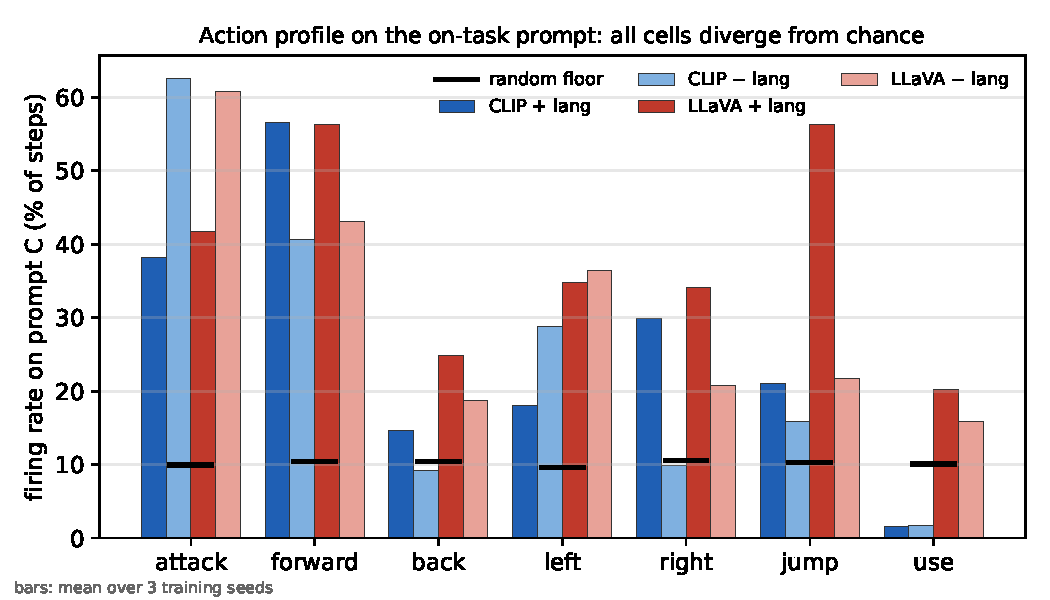
\includegraphics[width=0.92\textwidth]{figures/fig_action_profile.pdf}
\caption{Per-key firing rate on the on-task prompt (condition C) for the four
cells, against the random-policy floor (black ticks). All four trained cells
place most of their mass on \texttt{attack} and \texttt{forward}, several times
the $\sim\!10\%$ chance rate, so none is behaving randomly; they
differ in \emph{how} that mass is distributed.}
\label{fig:profile}
\end{figure}

\section{Language Conditioning}
\label{sec:exp-cond}

The central question of the prompt ablation is whether the language string
changes what the agent does. Table~\ref{tab:conditioning} reports the
\texttt{attack} and \texttt{forward} firing rates across the three chop-prompt
conditions, and Figure~\ref{fig:conditioning} plots the \texttt{attack} channel,
the most discriminative key.

\begin{table}[ht]
\centering
\begin{tabular}{llrrrrr}
\hline
Cell & Key & A (\%) & B (\%) & C (\%) & $\Delta_{\text{C}-\text{A}}$ (pp) & $h$ \\
\hline
Exp~2 CLIP + lang   & attack  & 84.9 & 76.7 & 37.0 & $-48.0$ & $-1.04$ \\
                    & forward & 76.3 & 71.2 & 62.6 & $-13.7$ & $-0.30$ \\
Exp~4 CLIP $-$ lang & attack  & 57.8 & 57.8 & 64.0 & $+6.1$  & $+0.13$ \\
                    & forward & 43.9 & 42.8 & 35.5 & $-8.4$  & $-0.17$ \\
Exp~1 LLaVA + lang  & attack  & 34.9 & 32.6 & 29.8 & $-5.1$  & $-0.11$ \\
                    & forward & 23.9 & 24.5 & 24.1 & $+0.2$  & $+0.00$ \\
Exp~3 LLaVA $-$ lang& attack  & 54.4 & 51.5 & 50.2 & $-4.2$  & $-0.09$ \\
                    & forward & 52.7 & 53.8 & 55.3 & $+2.6$  & $+0.05$ \\
\hline
\end{tabular}
\caption{Firing rates across the three chop-prompt conditions. $\Delta_{\text{C}
-\text{A}}$ is the on-task-minus-empty-prompt change in percentage points and
$h$ is Cohen's $h$ for that pair. Only CLIP + lang shows a large shift
($|h|>0.5$); the other three cells stay within $|h|\le0.17$, the same band as
the no-prompt controls.}
\label{tab:conditioning}
\end{table}

\begin{figure}[ht]
\centering
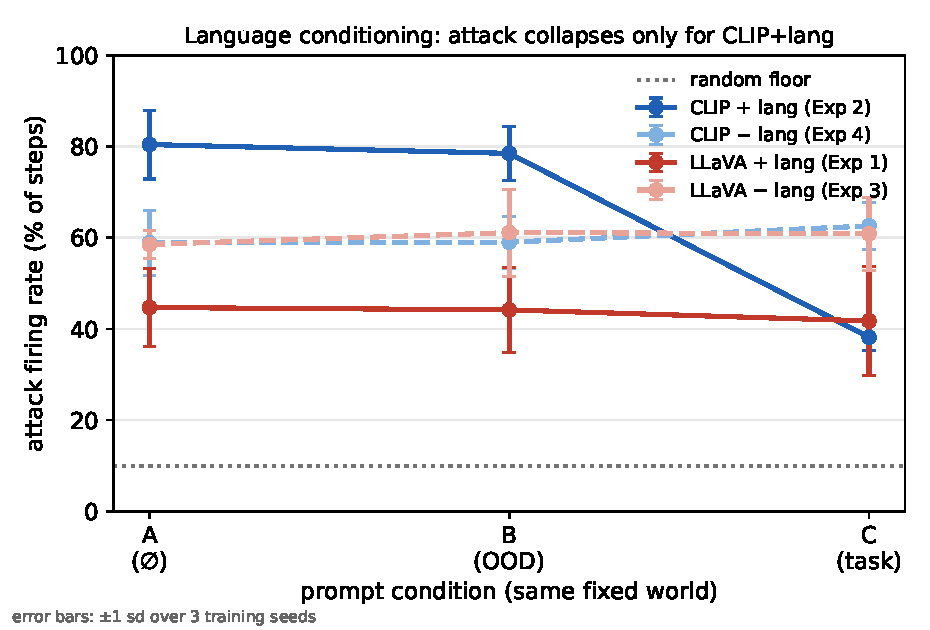
\includegraphics[width=0.82\textwidth]{figures/fig_conditioning.pdf}
\caption{\texttt{attack} firing rate across the empty (A), out-of-task (B) and
on-task (C) prompts; error bars are Wilson $95\%$ intervals (smaller than the
markers). Only CLIP + lang (solid blue) shifts with the prompt, its \texttt{attack}
rate moving from $84.9\%$ to $37.0\%$; the other three cells are flat, and all
sit well above the random floor (dotted).}
\label{fig:conditioning}
\end{figure}

The effect is large and concentrated in a single cell. \textbf{CLIP + lang}
suppresses its \texttt{attack} key from $84.9\%$ under the empty prompt to
$37.0\%$ under \enquote{chop a tree}, a $48$~percentage-point shift with
$h=-1.04$ --- a large effect by any threshold, and the prompt is the only
deliberately varied factor across the two conditions; with $\sim\!10^4$ steps per
condition the per-step intervals are far tighter than this shift, so it cannot be
attributed to rollout noise. The shift is not confined to one key: in the same
cell \texttt{sprint} falls by $29$~pp and rightward steering rises by $18$~pp
alongside the \texttt{forward} drop ($-13.7$~pp), whereas no other cell moves any
channel by more than about $6$~pp. The on-task prompt reorganises the whole
action distribution rather than nudging a single key. \textbf{CLIP $-$ lang}, the same
backbone with the text branch zeroed, is flat: \texttt{attack} moves by
$+6.1$~pp ($h=+0.13$), within the noise band, which is exactly the negative
control the design demands --- when language is removed from the representation,
the prompt string can no longer act.

Both LLaVA cells are flat in both conditions. \textbf{LLaVA + lang} shifts
\texttt{attack} by only $-5.1$~pp ($h=-0.11$) and \texttt{forward} not at all,
and \textbf{LLaVA $-$ lang} is indistinguishable from it ($-4.2$~pp). These
residual shifts reach nominal significance only because each rate is estimated
from $10^4$ steps; their effect sizes ($|h|<0.12$) sit inside the same band as
the no-prompt controls, so they carry no behavioural meaning. The asymmetry
noted in Section~\ref{ablation} sharpens rather than weakens this reading: in
the LLaVA no-prompt cell the prompt still passes through the decoder and only
the pooled text vector is zeroed, so the pooled image features remain
prompt-conditioned --- yet even with that residual pathway, and even with the
explicit text vector present in the prompt cell, LLaVA never separates from its
own control. The defensible conclusion is therefore a statement about the
backbone, not about language in general: \emph{under this frozen-feature regime
the contrastive CLIP text encoder yields a conditioning signal the head uses,
whereas the frozen LLaVA-1.5 backbone does not} --- and, as the probe of
Section~\ref{sec:exp-probe} shows, not because the prompt is absent from its
features but because the pooled representation does not expose it as an axis a
small head can act on.

\section{Task Performance}
\label{sec:exp-task}

Conditioning shows that a prompt changes behaviour; it does not show that the
behaviour completes the task. For task progress I use the reward-independent
peak-inventory measure of Section~\ref{sec:rollout}, the maximum count of the
goal item held during an episode. Chopping is at the floor for every cell ---
no cell collects more than a single log in any episode, in line with the broken
chop reward handler discussed in Section~\ref{sec:rollout} --- so the chop
conditions do not separate the models and I report dirt collection (condition D)
as the discriminating task. Table~\ref{tab:task} and Figure~\ref{fig:task} give
the per-episode results.

\begin{table}[ht]
\centering
\begin{tabular}{lrrrr}
\hline
Cell & dirt$_{\text{A}}$ (chop) & dirt$_{\text{D}}$ (dirt) & $95\%$ CI$_{\text{D}}$ & success$_{\text{D}}$ \\
\hline
Exp~2 CLIP + lang    & 0.8 & 4.30 & $[2.70,\,6.20]$ & $100\%$ \\
Exp~4 CLIP $-$ lang  & 2.5 & 2.30 & $[1.00,\,3.90]$ & $80\%$ \\
Exp~1 LLaVA + lang   & 0.0 & 0.00 & $[0.00,\,0.00]$ & $0\%$ \\
Exp~3 LLaVA $-$ lang & 0.9 & 0.10 & $[0.00,\,0.30]$ & $10\%$ \\
\hline
random policy        & 0.0 & 0.00 & --- & $0\%$ \\
\hline
\end{tabular}
\caption{Dirt collected per episode (mean peak inventory over $10$ episodes).
dirt$_{\text{A}}$ is \emph{incidental} digging in the chop environment under the
empty prompt; dirt$_{\text{D}}$ is digging in the dirt environment under the
on-task prompt. The interval is a $20{,}000$-resample percentile bootstrap of the
dirt$_{\text{D}}$ mean; success is the fraction of episodes collecting any dirt.
The dirt$_{\text{A}}$-versus-dirt$_{\text{D}}$ contrast separates goal-directed
digging from incidental terrain-attacking (see text).}
\label{tab:task}
\end{table}

\begin{figure}[ht]
\centering
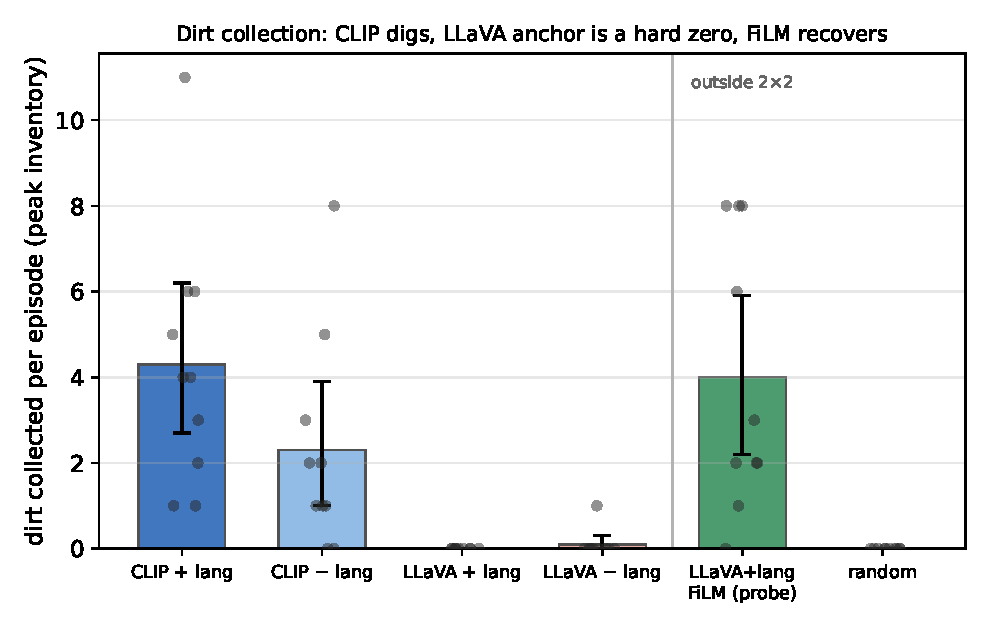
\includegraphics[width=0.92\textwidth]{figures/fig_taskperf.pdf}
\caption{Dirt collected per episode. Bars are means with percentile-bootstrap
$95\%$ intervals; grey dots are the ten individual episodes. The two CLIP cells
dig, the LLaVA anchor cells do not, and the random policy collects nothing. The
FiLM probe (green, right of the divider) lies outside the $2\times2$ and is
discussed in Section~\ref{sec:exp-film}.}
\label{fig:task}
\end{figure}

Task performance separates by backbone, not by language. \textbf{CLIP + lang}
collects $4.3$ dirt per episode and digs in every episode; \textbf{CLIP $-$
lang} collects $2.3$ and digs in eight of ten. Both LLaVA anchor cells are at
the floor: \textbf{LLaVA + lang} returns a hard zero across all ten episodes
(standard deviation $0$), and \textbf{LLaVA $-$ lang} reaches $0.1$ ---
indistinguishable from the random policy's zero. The CLIP--versus--LLaVA gap is
the one task comparison robust to the small sample: a cell that never collects
dirt in ten independent episodes is reliably below a cell that always does. The
within-CLIP gap between the prompt and no-prompt cells ($4.3$ versus $2.3$) is
in the expected direction but \emph{soft}: the two confidence intervals overlap,
so with ten episodes I cannot claim the prompt improves dirt collection; the two
cells are statistically indistinguishable on this metric at this sample size.
This is the honest limit of episode-level metrics at
the sample size the LLaVA backbone makes affordable, and it is why the
conditioning analysis of Section~\ref{sec:exp-cond}, which rests on $10^4$
per-step observations, carries the load-bearing claim.

One caveat on this metric matters, because the dirt count is not a pure measure
of goal pursuit. Comparing the two leftmost columns of Table~\ref{tab:task},
\textbf{CLIP + lang} collects only $0.8$ dirt incidentally in the \emph{chop}
environment but $4.3$ when actually told to collect dirt --- a genuine,
prompt-and-task-driven lift. \textbf{CLIP $-$ lang}, by contrast, digs essentially
the same amount in both environments ($2.5$ versus $2.3$): its dirt comes from
indiscriminately attacking the ground, not from pursuing the goal. Read this way
the task result is sharper than a raw ranking suggests --- it is specifically the
\emph{prompted} CLIP agent whose digging tracks the instruction, the same
conditioning signal of Section~\ref{sec:exp-cond} now visible in an item count
rather than a firing rate --- and it is the prompt-driven lift between
environments, not the absolute count, that cleanly measures task-following.

\section{Offline Frame Metrics and the Offline--Online Gap}
\label{sec:exp-offline}

The rollout results stand in sharp contrast to how the four cells look on the
held-out test frames of Section~\ref{sec:split}. Table~\ref{tab:offline} reports
the offline metrics over $1{,}252{,}328$ test frames per cell. On frames the four
cells are near-indistinguishable: binary-key accuracy is $0.98$ for all four,
\texttt{attack}-$F_1$ is $0.96$, camera bin accuracy is $0.87$ (against a
majority-class, always-still baseline of roughly $78\%$) and camera error is
below half a degree. Even the most behaviourally relevant offline number, the
movement-$F_1$ that selects the checkpoint (Section~\ref{caching}), spans only
$0.368$ to $0.431$ across the four --- and ranks them in an order the rollouts
flatly contradict: \textbf{CLIP $-$ lang} has the \emph{highest} movement-$F_1$
($0.431$) yet collects half the dirt of \textbf{CLIP + lang}, and \textbf{LLaVA
$-$ lang} ($0.368$) sits within $0.04$ of \textbf{CLIP + lang} ($0.407$) yet
collects nothing.

\begin{table}[ht]
\centering
\begin{tabular}{lrrrrr}
\hline
Cell & binary acc & \texttt{attack} $F_1$ & movement $F_1$ & camera acc & camera MAE ($^\circ$) \\
\hline
Exp~2 CLIP + lang    & 0.982 & 0.964 & 0.407 & 0.869 & 0.48 \\
Exp~4 CLIP $-$ lang  & 0.982 & 0.964 & 0.431 & 0.869 & 0.48 \\
Exp~1 LLaVA + lang   & 0.981 & 0.962 & 0.369 & 0.868 & 0.48 \\
Exp~3 LLaVA $-$ lang & 0.981 & 0.962 & 0.368 & 0.868 & 0.49 \\
\hline
\end{tabular}
\caption{Offline frame-level metrics on the held-out test split
($1{,}252{,}328$ frames per cell). Binary accuracy is averaged over the $21$
keys; movement-$F_1$ is the mean $F_1$ over the locomotion keys (the
model-selection criterion of Section~\ref{caching}); camera accuracy is top-1
mu-law bin accuracy on \texttt{camera\_x}. The four cells are a near-tie, and
movement-$F_1$ even ranks CLIP $-$ lang above CLIP + lang --- the reverse of the
rollout ranking.}
\label{tab:offline}
\end{table}

\begin{figure}[ht]
\centering
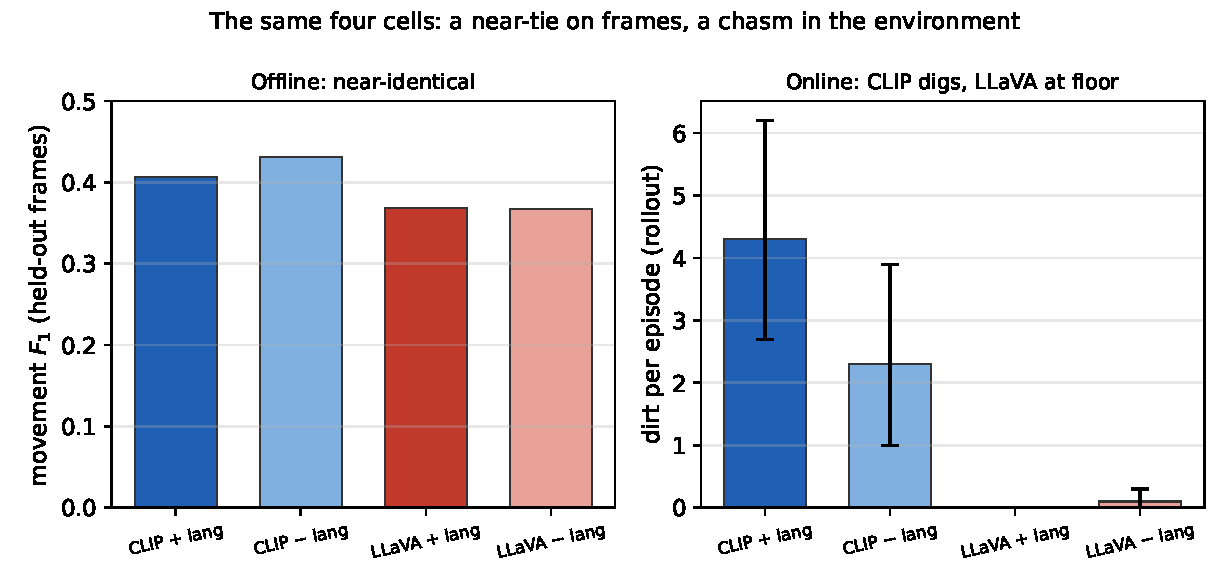
\includegraphics[width=0.95\textwidth]{figures/fig_dissociation.pdf}
\caption{The same four cells, measured two ways. \emph{Left:} movement-$F_1$ on
held-out frames --- a near-tie, with CLIP $-$ lang nominally highest.
\emph{Right:} dirt collected per rollout episode (percentile-bootstrap $95\%$
intervals) --- CLIP digs, both LLaVA cells are at the floor. Frame accuracy does
not predict in-environment behaviour.}
\label{fig:dissociation}
\end{figure}

This offline--online dissociation is the empirical core of the thesis's third
contribution. Held-out frame accuracy --- the metric most imitation-learning work
reports --- would rank these four backbones as interchangeable and would miss the
entire conditioning and task-collection story that appears only once the policy
is closed in the loop. It is a concrete instance of the known weak correlation
between offline action metrics and downstream task success~\cite{kanervisto2020}:
a single mispredicted key every few steps, invisible at the frame level, compounds
over a thousand-step episode into the difference between digging a stack of dirt
and digging nothing. The rollout evaluation is therefore not a costlier
restatement of the frame metrics but a qualitatively different measurement --- and
it is the one that separates the backbones.

\section{Features or Head? A FiLM Probe}
\label{sec:exp-film}

Read on its own, Section~\ref{sec:exp-task} invites the conclusion that the
frozen LLaVA features are useless for control. That conclusion would be too
strong, and a single departure from the $2\times2$ shows why. The LLaVA anchor
feeds the pooled text vector to the head by plain concatenation
(Section~\ref{action_head}); if the head instead conditions on that vector
through feature-wise linear modulation (FiLM), so that the text representation
\emph{scales and shifts} the visual features rather than sitting beside them,
the same frozen LLaVA + lang features that produced a hard zero now collect
$4.0$ dirt per episode at $90\%$ success --- comparable to the best CLIP cell
($4.3$), with the two means well within each other's confidence intervals. The frozen LLaVA
representation therefore \emph{does} carry the information needed to dig; the
anchor's failure is a read-out failure in the head, not an absence of signal in
the features.

Two caveats keep this a probe rather than a result. It is a single architectural
change evaluated on ten episodes, with no matched no-prompt FiLM control, so it
sits deliberately outside the controlled $2\times2$. And it does not recover
conditioning: the FiLM cell still shifts \texttt{attack} by only $+3$~pp between
the empty and on-task prompts, as flat as every other LLaVA cell. A better head
unlocks the \emph{task} signal in the LLaVA features but not a prompt-driven
\emph{conditioning} signal. That a head which multiplicatively gates the visual
features on the text vector still does not condition is itself informative: it
indicates the limit is not head capacity but the pooled text representation, which
does not expose a prompt axis to gate on (Section~\ref{sec:exp-probe}). I return to
the implications of this split in Chapter~\ref{chap:discussion}.

\section{Is the Prompt Represented? A Linear Probe}
\label{sec:exp-probe}

Is the LLaVA conditioning failure a missing signal or an unusable one? A cheap
offline probe narrows it down. On the cached training features I fit a logistic
regression to predict the task --- equivalently, which training prompt was given
--- from the image half of the pooled feature, the text half, and the full
vector, on a balanced $30{,}000$-frame sample (Table~\ref{tab:probe}).

The task is almost perfectly decodable from the pooled LLaVA text half ($99.7\%$),
above the $90.1\%$ reachable from the image half, and it collapses to chance
($50\%$) when the text half is zeroed: the prompt is far from washed out of the
representation. But decodability alone does not make the prompt \emph{usable} for
conditioning, because in the combined training set the two prompts are perfectly
correlated with two visual distributions (forest versus plains) and the pooled
LLaVA text half is image-entangled --- its tokens attend to the frame inside the
decoder. The probe cannot separate a genuine prompt axis from the image content
that leaks into the text positions.

\begin{table}[ht]
\centering
\begin{tabular}{lrrr}
\hline
Cache (probe input) & image & text & full \\
\hline
CLIP + lang ($768/768$)        & 98.3 & 100.0 & 100.0 \\
LLaVA + lang ($4096/4096$)     & 90.1 & 99.7  & 99.3 \\
LLaVA $-$ lang (text zeroed)   & 89.9 & 50.0  & 90.0 \\
\hline
\end{tabular}
\caption{Task-decoding accuracy (\%) of a logistic probe predicting the task
(chop vs dirt, i.e.\ which prompt was given) from each half of the pooled feature
($30{,}000$ balanced frames, $70/30$ split). The LLaVA text half encodes the
prompt almost perfectly, refuting a literally \enquote{washed-out} reading; the
no-prompt control, whose text half is zeroed, drops to chance.}
\label{tab:probe}
\end{table}

Which it is --- a usable axis or a confound --- is settled by the FiLM result.
A head that multiplicatively gates on exactly this text vector
(Section~\ref{sec:exp-film}) is a more expressive way to condition than the
concatenating head, yet it produces no behavioural shift ($+3$~pp). Were the text
half a clean, prompt-isolated axis, such a head would ride it; that it does not
indicates the decodable direction is largely the prompt--image confound rather
than a separable prompt signal. The contrast with CLIP makes this concrete: CLIP's
text encoder is physically separate from its image encoder, so its prompt
embedding is image-independent and moves when, and only when, the prompt changes
--- the axis the head learns to use. The bottleneck for LLaVA is therefore not
that the head is too weak but that its pooled, image-entangled text representation
does not present a prompt axis to act on; the limit sits upstream of the head. A
counterfactual test that changes only the prompt at a fixed frame would measure
the confound directly, and is left to Chapter~\ref{chap:discussion}.

\section{Summary of Findings}
\label{sec:exp-summary}

\begin{itemize}
\item All four cells diverge sharply from a random policy, which fires every key
at $\sim\!10\%$ and collects nothing; the trained agents are genuine policies,
not noise (Figure~\ref{fig:profile}).
\item Language conditioning is a backbone effect. Only CLIP + lang reshapes its
policy with the prompt (\texttt{attack} $-48$~pp, $h=-1.04$); its no-prompt
control and both LLaVA cells stay within the $|h|\le0.17$ noise band
(Table~\ref{tab:conditioning}). The prompt is not missing from LLaVA's features
--- a linear probe recovers the task from its pooled text half at $99.7\%$
(Section~\ref{sec:exp-probe}) --- but it is entangled with the image, and no
head-side lever, the FiLM gate included, turns it into conditioning; the
bottleneck is the pooled representation, not the head.
\item Task performance also separates by backbone: CLIP collects dirt ($4.3$ and
$2.3$ per episode) while both LLaVA anchor cells are at the floor
(Table~\ref{tab:task}). The within-CLIP prompt effect is in the right direction
but not significant at ten episodes; chopping fails for every model. The dirt
count is partly confounded by incidental digging, but it is the prompt-driven
\emph{lift} between environments that is goal-directed, and that lift appears only
for CLIP + lang.
\item Held-out frame metrics do not predict rollout behaviour: all four cells
score within $0.04$ movement-$F_1$ and $0.001$ binary accuracy offline, yet
diverge from $4.3$ to $0$ dirt online --- a direct demonstration that rollout
evaluation measures what frame metrics miss
(Section~\ref{sec:exp-offline}, Figure~\ref{fig:dissociation}).
\item The LLaVA floor is a head limitation, not a feature limitation: a
FiLM-conditioned head lifts dirt collection from zero to $4.0$ per episode,
comparable to the CLIP cells, from the same frozen features, without recovering conditioning
(Section~\ref{sec:exp-film}).
\end{itemize}

\chapter{Discussion}
\label{chap:discussion}

The objective of this thesis was to find an effective yet cheap recipe for
turning a pretrained vision-language model into an acting agent, using Minecraft
as a deliberately hard test bed. The recipe was held to two constraints: the
backbone stays frozen, and training stays inexpensive enough to sweep the full
ablation on a single rented GPU (Section~\ref{caching}). This chapter reads the
results of Chapter~\ref{chap:experiments} against that objective, asks why the
two backbones behave so differently, examines what the agents do and do not
achieve in the chop environment, states the limits of the study, and lays out
two directions the findings open up.

\section{CLIP and LLaVA Head-to-Head Under a Cheap, Frozen Regime}
\label{sec:disc-headtohead}

The clearest message of the ablation is that, under the constraints this thesis
imposes, the simpler backbone wins --- with the important qualification,
developed below, that this is a property of the minimal head, not an intrinsic
ranking of the two backbones. Of the two frozen extractors, the
contrastive CLIP encoder both conditions on the prompt
(Section~\ref{sec:exp-cond}) and collects the discriminating item
(Section~\ref{sec:exp-task}), whereas the joint LLaVA-1.5 backbone does neither
in its matched, knob-free configuration. On the task that separates the cells,
dirt collection, CLIP digs reliably with and without the prompt ($2.53$ and
$1.60$ per episode, averaged over three training seeds) while both LLaVA anchor
cells sit at the floor ($0.07$, $0.47$); on conditioning, CLIP with language
shifts its \texttt{attack} rate by $42$ percentage points between the empty and
on-task prompts, an effect an order of magnitude larger than anything either
LLaVA cell produces and present in all three seeds. For a practitioner who wants
a controllable short-horizon agent on a small budget, the result is encouraging:
the cheaper $0.43$B contrastive encoder, paired with a $4.6$M-parameter head, is
the more effective choice here \emph{under this minimal head}, not the $7$B
autoregressive one. Set against the contractor it imitates, though, even the best
agent is modest in absolute terms: measured from the recordings, the demonstrator
collects $18.3$ dirt per thousand steps, so CLIP\,+\,lang's $2.5$ is about a
seventh of the expert rate --- far above the random floor of zero, but a reminder
that the comparison this study makes cleanly is between cells, not against
mastery.

This separation is invisible to held-out frame accuracy. On the test frames the
four cells are near-identical --- movement-$F_1$ spans only $0.368$ to $0.431$ and
even ranks CLIP $-$ lang first --- yet they diverge from a dug stack of dirt to
nothing in rollout (Section~\ref{sec:exp-offline}). The head-to-head verdict is therefore a
property of closed-loop behaviour, not of frame-level fit, and it would be missed
entirely by the offline metrics that imitation-learning studies usually report.
This is itself the answer to the third research question, and a caution against
selecting backbones on frame accuracy alone.

This conclusion must be stated at the right altitude, and the FiLM probe of
Section~\ref{sec:exp-film} fixes that altitude. The probe shows that the same
frozen LLaVA features that produced a hard zero can be made to collect dirt at
CLIP-comparable levels once the head reads them through feature-wise modulation
rather than plain concatenation. The honest claim is therefore not that LLaVA's
representation is intrinsically weaker for control, but that \emph{under the
simplest head---the one the controlled $2\times2$ holds fixed---CLIP extracts
more usable task signal per unit of engineering effort}. The advantage CLIP
shows is an advantage of the cheap regime, which is precisely the regime this
thesis set out to characterise. A contrastive encoder aligns image and text in a
single shared embedding by construction, so a linear head can read a
prompt-dependent direction out of it directly; the joint decoder hides the same
information behind a pooling and read-out step that the minimal head cannot
invert.

\section{Why the LLaVA Language Pathway Stays Silent}
\label{sec:disc-washout}

The most striking negative result is that LLaVA's behaviour is statistically
indistinguishable across all four prompt conditions: the explicit task string
moves the policy no more than the zeroed control does. The tempting reading ---
that the language tokens are drowned out by the roughly $576$ image tokens --- is
too crude. The \texttt{<image>} placeholder is expanded into those visual tokens
\emph{alongside} the prompt tokens, the split-pooling of Section~\ref{sec:backbone}
keeps the text-role tokens as an explicit half of the feature, and the linear
probe of Section~\ref{sec:exp-probe} shows the prompt is in fact almost perfectly
recoverable from that half ($99.7\%$, collapsing to chance when it is zeroed). The
prompt is not washed out in the crude sense.

Recoverable, however, is not the same as usable, and the rest of the evidence
shows the limit is the representation, not the head. In the combined training set
the two prompts are perfectly correlated with the two tasks' imagery
(tree-felling versus dirt-digging scenes), and the pooled LLaVA text half is
image-entangled --- its tokens attend to the frame inside the decoder --- so the
$99.7\%$ is largely a prompt--image confound rather than a clean prompt axis. The
rollout evaluation breaks that correlation: it issues all four prompts in one
fixed scene (Section~\ref{sec:exp-setup}), so prompt and image are decorrelated,
and the LLaVA policy still does not move --- the prompt axis is absent there, not
merely masked by the image. Two converging checks confirm the limit is upstream
of the head rather than in it. First, a FiLM head that multiplicatively gates the
features on that very text vector, strictly more expressive than the concatenating
baseline, still does not condition (Section~\ref{sec:exp-film}); if a usable
prompt axis were present a gating head would exploit it. Second, that same gating
head, and a second alternative read-out, \emph{do} recover the dirt \emph{task}
from the identical features --- so the heads are capable enough to use what the
representation exposes, and what it exposes is task identity, not a steerable
prompt direction. Head capacity is therefore not the limiting factor. The contrast
with CLIP isolates what is: CLIP's text encoder is physically separate from its
image encoder, so its prompt embedding is an image-independent axis that moves
when, and only when, the prompt changes, and the head learns to ride it. LLaVA's
final-layer text positions, mean-pooled, fold the prompt and the frame together,
so changing only the prompt at a fixed scene barely moves the representation. The
bottleneck is thus upstream of the head, and the remedies that follow are
representational rather than architectural on the head side: pooling the prompt
from a position that is not image-saturated --- the final text token rather than
the mean --- or lightly fine-tuning the backbone so the text pathway carries a
separable signal. A counterfactual probe that swaps the prompt at a fixed frame
measures this directly (Section~\ref{sec:exp-probe}): LLaVA's pooled text half
barely moves under the swap (cosine $1.00$) while CLIP's moves substantially
(cosine $0.74$), confirming that the limit is the representation, not the head.

\section{Targeting Without Completion in the Chop Environment}
\label{sec:disc-chop}

Reward and item counts tell only part of the story for the chop task, where every
cell is at the floor (Section~\ref{sec:exp-task}). Inspecting the rollout videos
rather than the scalar logs reveals that the better CLIP agents are not failing
at random: they orient toward nearby trees, walk up to a trunk, and fire
\texttt{attack} into it --- the coarse structure of chopping is present. What they
miss is the fine control that finishes the job: holding the camera steady on a
single block long enough, at the right pitch, for the break to complete. The
agent targets the tree but does not reliably mine the block. This is the
signature of the compounding-error ceiling that behavioural cloning carries by
construction (Section~\ref{sec:bg-il}): trained only to imitate single-step
actions with no reward and no corrective feedback, the policy reproduces the
gross demonstrated behaviour but drifts on the tight closed-loop control that
block-breaking demands, and nothing in the offline objective pushes it back onto
the narrow trajectory that completes the chop. A demo-side analysis locates where
that trajectory runs out of supervision. Aligning camera motion to the onset of
sustained \texttt{attack} runs --- the median chop commit lasts about $90$ frames
--- shows the contractor does move the camera more in the half-second \emph{before}
committing to a chop than during it ($3.1^\circ$ versus $1.4^\circ$ of per-frame
motion), so an aiming phase is present in the data. But that motion is largely
undirected: its net signed pitch is only $-0.45^\circ$ against $1.4^\circ$ of
magnitude --- a faint downward bias toward the trunk base, swamped by exploratory
wander --- and yaw carries no consistent direction at all. The precise
\enquote{aim at the trunk} signal a head would need to finish the block is
therefore weak in the demonstrations themselves, so part of the chop gap is a
limit of the supervision, not only of the cloned policy. That the qualitative
behaviour is already on the right track, while the scalar reward stays at zero, is itself a
finding: it suggests the gap to task completion here is one of refinement, not of
gross capability, and that the right lever is a training signal that can reward
the last few degrees of aim rather than a larger or unfrozen backbone.

The conditioning result of Section~\ref{sec:exp-cond} casts this task in a second,
initially puzzling light: the on-task \enquote{chop a tree} prompt \emph{suppresses}
the CLIP\,+\,lang agent's \texttt{attack} key, from $80.4\%$ under the empty prompt
to $38.2\%$ --- a drop in precisely the action that chopping requires. A natural
hope is that this merely replays the demonstrations, but the contractor data rules
that out. Measured directly from the recordings, the chop demonstrator attacks on
$83.1\%$ of steps and the dirt demonstrator on $94.6\%$; both tasks are
attack-heavy, and the empty-prompt policy ($80.4\%$) faithfully reproduces that
baseline. The prompt then drives \texttt{attack} \emph{below} either demonstrator,
so the suppression cannot be imitation of a low-attack chopping style --- no such
style exists in the data. It is a genuine prompt-induced reorganisation of
behaviour rather than a replayed statistic; what it is not is evidence of
\emph{correct} task behaviour, since neither the high-attack empty-prompt agent nor
the suppressed prompted one completes a chop. The $42$-point shift thus shows that
the prompt steers the policy (RQ2) without showing that it steers it toward the
goal: the chop environment exposes the limit of conditioning as sharply as the
dirt environment exposes its use, and steering and task-appropriateness remain
separate properties.

\section{Limitations}
\label{sec:disc-limits}

Several limits bound how far these conclusions generalise. First, the
in-environment comparisons rest on ten episodes per cell per training seed;
although MineRL is seed-deterministic, so each run reproduces exactly, ten
episodes is still a small sample over ten distinct world seeds. The per-step
firing rates that carry the conditioning result are estimated from
$\sim\!3\times10^4$ pooled observations and are robust, but the per-episode task
metrics are noisier, so the within-CLIP prompt-versus-no-prompt difference is only
suggestive and the cross-backbone task gap is the one task comparison I treat as
reliable. To bound the training-side counterpart of this caveat, each cell is
trained at three independent seeds (head initialisation and data-order shuffle);
the headline effects survive it. The conditioning shift is $-42.3\pm10.4$ points
and large in every seed ($h=-1.04,-1.12,-0.57$); the LLaVA flats are symmetric
across all three seeds ($|h|\le0.16$); and the cross-backbone dirt gap holds (CLIP
$2.53\pm1.25$ and $1.60\pm0.50$ versus the LLaVA anchors' $0.07$ and $0.47$). What
three seeds reveal, and a single seed hid, is that several absolute numbers were
seed-lucky: CLIP\,+\,lang's dirt count was $4.3$ in the original seed but
$2.53\pm1.25$ across seeds, and the FiLM task recovery likewise. The signs and
orderings are stable; the precise magnitudes should be read with their across-seed
spread. The quantitative \emph{task} story, in turn, rests on a single working
task: chop is at the floor for every cell, so dirt collection is the only task on
which the agents produce a completion metric at all, with the chop environment
contributing the per-step conditioning shift and the qualitative targeting result
but no scalar separation. Second, the study fixes the
backbone as frozen and the head as a minimal two-layer MLP; it therefore
characterises the cheap-and-frozen corner of the design space and cannot speak to
what either backbone achieves under fine-tuning or a richer head, a boundary the
FiLM probe already shows matters. Third, the policy is single-frame with a short
past-action window, so it is structurally ill-suited to the long-horizon credit
assignment that full task completion in Minecraft demands. Fourth, the two tasks
are short-horizon and the prompt doubles as a task-identity signal on the combined
dataset (Section~\ref{ablation}), so the conditioning result demonstrates that
language \emph{routes behaviour by task} for CLIP, not that the model parses
compositional instructions. Relatedly, the dirt-collection metric is not a pure
measure of goal pursuit: every cell digs some dirt incidentally, by attacking the
ground, even under the empty prompt and in the same fixed world
(Table~\ref{tab:task}), so an absolute dirt count conflates goal-directed digging
with incidental ground-attacking. The prompt-driven component is visible only for
CLIP\,+\,lang, and even there it is weak and seed-variable at the episode level
(an empty-to-dirt-prompt lift of $1.4\pm1.7$), which is why the reproducible
prompt-steering evidence is the per-step firing-rate conditioning, not the item
count. Finally, the LLaVA no-prompt control is not a perfect
negative: because the prompt still flows through the decoder and only the pooled
text vector is zeroed, the LLaVA image features remain prompt-conditioned even in
the control, which is one more reason the cleanest statement is the
\emph{symmetric} flatness of LLaVA across all four conditions rather than a single
prompt-versus-control contrast.

\section{Future Directions}
\label{sec:disc-future}

The findings push in two complementary directions.

\paragraph{Earn the joint backbone its keep.} The silence of LLaVA's language
pathway is a property of the frozen, minimal-head regime, not a verdict on joint
vision-language models, which have driven strong long-horizon Minecraft and
robotics agents once a heavier pipeline is allowed
\cite{li2025jarvisvla, kim2024openvla, brohan2023rt2, black2024pi0}. Because the
bottleneck this study locates is upstream of the head, in the pooled text
representation (Section~\ref{sec:disc-washout}), the cheapest next step keeps the
whole two-stage pipeline and changes only how the prompt is pooled: re-caching from
a position that is not image-saturated --- the final text token rather than the
mean over text positions --- might expose the prompt as a separable axis at no
extra training cost. Beyond that, relaxing the freeze with parameter-efficient
fine-tuning such as LoRA \cite{hu2022lora}, or a few learnable conditioning tokens,
could let the decoder carry a behaviourally separable prompt signal without the
feature distortion that full fine-tuning risks
\cite{kumar2022finetuningdistortpretrainedfeatures, simchowitz2025pitfalls}.
These remedies are now well motivated rather than speculative, because the
counterfactual prompt-swap probe of Section~\ref{sec:exp-probe} has confirmed
their target directly: holding the frame fixed and swapping only the prompt moves
LLaVA's pooled text half by a mere one percent (cosine $1.00$), against CLIP's
substantial swing (cosine $0.74$), so the prompt does not register in LLaVA's
pooled representation at all. The fix must therefore act on that representation ---
re-pooling from the final text token or relaxing the freeze so the text pathway
carries a prompt-separable signal --- and the same probe gives a cheap acceptance
test for whether it worked: a successful intervention should raise the LLaVA
prompt-swap displacement toward CLIP's before any head is retrained.

\paragraph{Lean into cheap models, and compose them.} The other direction takes
the CLIP result at face value: a small contrastive backbone with a light head is
already an effective short-horizon controller, so it is worth pushing how far that
cheapness scales. Long-horizon competence need not come from a single large model;
it can come from composing several cheap, prompt-conditioned CLIP heads into a
multi-skill policy that is directed by a separate language model acting as a
high-level planner \cite{lifshitz2023steve1, fan2022minedojo, lynch2021langlfp}.
Such a hierarchy keeps each control policy simple and inexpensive to train while
letting the planner supply the knowledge-based reasoning that bridges abstract
goals and low-level actions --- exactly the gap a frozen contrastive encoder
cannot close on its own.

\paragraph{Close the loop with reward.} Cutting across both directions is the
chop observation of Section~\ref{sec:disc-chop}: a behaviourally-cloned CLIP agent
that already targets trees but cannot finish the block is a strong starting point
for a second, online training stage. Fine-tuning the cloned policy against a
rollout-based reward, or nudging it with corrective feedback in the
DAgger family \cite{ross2011}, would supply exactly the closed-loop signal that
offline cloning lacks, reinforcing the last few degrees of aim that separate
visible targeting from a completed chop. Because the underlying gross behaviour is
already present, such a stage plausibly needs far less interaction than learning
the task from scratch --- a hypothesis that follows directly from the qualitative
result and that the cheap-and-frozen recipe of this thesis is well positioned to
seed.

\chapter{Conclusion and Future Work}
\label{chap:conclusion}

This thesis asked whether a frozen, general-purpose vision-language model can be
turned into a controllable Minecraft agent cheaply --- by training only a small
action head with behavioural cloning, holding the backbone fixed and keeping the
whole ablation inexpensive enough to sweep on a single rented GPU. Using a
$2\times2$ ablation over backbone (LLaVA-1.5 versus CLIP) and language condition,
evaluated in live MineRL rollouts, it reached a clear and slightly surprising
answer: in this cheap, frozen regime the contrastive backbone is the more
effective and the more language-steerable choice \emph{under a minimal head} --- a
richer (FiLM) read-out narrows the task gap from the same LLaVA features, so the
backbone finding is best read as a head-readout-by-backbone interaction rather
than an intrinsic ranking of the two models.

Table~\ref{tab:contributions} maps each research question of
Chapter~\ref{chap:intro} to the evidence that settles it.

\begin{table}[ht]
\centering
\begin{tabular}{p{0.11\textwidth}p{0.38\textwidth}p{0.40\textwidth}}
\hline
 & Question & Finding \\
\hline
RQ1 \newline (backbone) & Used only as a frozen extractor, does a joint VLM beat
a contrastive one? & \textbf{No}, in this regime. CLIP collects $2.5$ dirt per
episode where the matched LLaVA cell is at the floor ($0.07$); the gap is a
read-out effect, since two alternative heads (FiLM, fixAB) recover CLIP-level
collection from the same LLaVA features
(Sections~\ref{sec:exp-task}, \ref{sec:exp-film}). \\
RQ2 \newline (language) & Does the prompt change behaviour, and does it depend on
the backbone? & \textbf{Yes}, and it depends entirely on the backbone. Only
CLIP + lang shifts (\texttt{attack} $-42\pm10$~pp, $h=-0.91$, in all three seeds);
both LLaVA cells and the CLIP control are flat (Section~\ref{sec:exp-cond}). The
prompt \emph{steers} behaviour but not necessarily toward the goal --- the robust
shift is a \emph{suppression} of the action chopping needs
(Section~\ref{sec:disc-chop}). \\
RQ3 \newline (evaluation) & Do rollouts reveal what frame metrics miss? &
\textbf{Yes}, decisively. The four cells are a near-tie on held-out frames yet
diverge from a dug stack of dirt to nothing in rollout
(Section~\ref{sec:exp-offline}). \\
\hline
\end{tabular}
\caption{The three research questions and the evidence that settles each.}
\label{tab:contributions}
\end{table}

Two interpretive points carry beyond the table. First, the LLaVA result is a
statement about the cheap-and-frozen regime, not about the backbone's ceiling: its
pooled text representation in fact encodes the prompt almost perfectly (a linear
probe recovers it at $99.7\%$), but in a form entangled with the image that no
head-side lever --- including a feature-gating FiLM head --- converts into
conditioning, so the bottleneck is the pooled representation and the fix is
upstream of the head (Chapter~\ref{chap:discussion}). Its visual features,
meanwhile, are usable for the task itself once the head reads them through
modulation rather than concatenation. Second, the conditioning result is a
behaviour-routing effect shown on two short-horizon tasks with the prompt doubling
as task identity; it should not be over-read as compositional
instruction-following, and absolute dirt counts mix goal-directed digging with
incidental terrain-attacking (Section~\ref{sec:exp-task}). Within those bounds the
central claim is firm: under a fixed, inexpensive training budget, a frozen
contrastive encoder with a five-million-parameter head is both a more effective
short-horizon Minecraft controller and a more language-steerable one than a frozen
seven-billion-parameter joint model \emph{read through the same minimal head}. The
task half of that gap is a head-readout effect --- a FiLM head recovers it from the
LLaVA features --- so the claim is about the cheap regime and its default
read-out, not about the backbones' intrinsic limits.

\paragraph{Outlook.} Chapter~\ref{chap:discussion} develops three directions in
detail. The first relaxes the freezing constraint on the joint backbone exactly
where this study located the bottleneck --- the entangled text representation ---
through parameter-efficient fine-tuning or a few learnable conditioning tokens,
paired with a direct representational probe to confirm whether the text features
then separate by task. The second takes the CLIP result at face value and composes
several cheap, prompt-conditioned heads into an LLM-directed hierarchy, keeping
each controller small while a planner supplies the long-horizon reasoning. The
third closes the loop with reward: the chop rollouts show a cloned CLIP agent that
already targets trees but cannot finish the block, an ideal starting point for an
online, reward-based refinement stage. The cheap-and-frozen recipe characterised
here is a natural seed for all three.








\newread\tmp

\newcommand{\quickcharcount}[1]{%
  \immediate\write18{texcount -1 -sum -merge -char #1.tex > #1-chars.sum}%
  \openin\tmp=#1-chars.sum%
  \read\tmp to \thechar%
  \closein\tmp%
}

\newcommand{\quickwordcount}[1]{%
  \immediate\write18{texcount -1 -sum -merge #1.tex > #1-words.sum}%
  \openin\tmp=#1-words.sum%
  \read\tmp to \theword%
  \closein\tmp%
}


\quickwordcount{main}
\quickcharcount{main}

There are \thechar characters and approximately \theword spaces.
That makes approximately \the\numexpr\theword+\thechar\relax\ characters total.


%% Ende Hauptteil

% Abbildungsverzeichnis (kann auch nach dem Inhaltsverzeichnis kommen)
%\listoffigures

% Tabellenverzeichnis (kann auch nach dem Inhaltsverzeichnis kommen)
%\listoftables

% Literaturverzeichnis
\bibliographystyle{plain}
\bibliography{dbstmpl}


% verwendet dbstmpl.bib

\end{document}
